\documentclass[11pt,a4paper,oneside]{bth}
\usepackage{setspace}
\usepackage{tocloft}

\usepackage[pagestyles]{titlesec}

\usepackage{enumitem}

\usepackage{hyperref}

%%%%


\usepackage{textcomp}
\usepackage{longtable}
\usepackage{multirow}
\usepackage{pifont}
\usepackage{changepage}
\usepackage{listings}
\usepackage{graphicx}
%\DeclareGraphicsExtensions{.pdf}

\usepackage{biblatex}
\addbibresource{ref.bib}

\usepackage{lipsum}       % for sample text
\usepackage{changepage}   % for the adjustwidth environment

\usepackage{wrapfig}







\graphicspath{ {./images/} }

%%%%

%\usepackage{showframe}% http://ctan.org/pkg/showframe
%\usepackage{etoolbox}% http://ctan.org/pkg/etoolbox

\hoffset = 0pt
\voffset = 0pt

\topmargin= 0in
\headheight=15pt
\headsep=30pt
\parindent=0pt

\marginparwidth = 5pt
\marginparsep = 10pt


\titleformat{\chapter}[display]
   {\normalfont\huge\bfseries\centering}{\centering\chaptertitlename\ \thechapter}{10pt}{\Huge}
\titlespacing*{\chapter}
   {0pt}{0pt}{25pt}


\makeatletter
\@addtoreset{section}{part}
\makeatother
\newlength\mylen

\renewcommand\thepart{\Roman{part}}
\renewcommand\thechapter{\arabic{chapter}}
\renewcommand\thesection{\Roman{section}}
\renewcommand\thesubsection{(\arabic{subsection})}

\renewcommand\cftpartpresnum{Part~}
\settowidth\mylen{\bfseries\cftpartpresnum\cftpartaftersnum}
\addtolength\cftpartnumwidth{\mylen}

\setlength{\cftbeforetoctitleskip}{-3em}


\newlist{abbrv}{itemize}{1}
\setlist[abbrv,1]{label=,labelwidth=1in,align=parleft,itemsep=0.1\baselineskip,leftmargin=!}

\usepackage{graphicx,array}
\newcolumntype{C}[1]{>{\centering\let\newline\\\arraybackslash\hspace{0pt}}m{#1}}
\newcolumntype{L}[1]{>{\raggedright\let\newline\\\arraybackslash\hspace{0pt}}m{#1}}

\hypersetup{%
    %pdfpagemode={UseOutlines},
    bookmarksopen,
    pdfstartview={FitH},
    colorlinks,
    linkcolor={black},
    citecolor={blue},
    urlcolor={blue}
  }
 



\begin{document}

\pagestyle{plain}
\pagenumbering{arabic}


% Front matter


{\pagestyle{empty}
\changepage{4.5cm}{2.5cm}{-0.5cm}{-1cm}{}{-2cm}{}{}{}
\noindent%
{\large
\begin{tabular}{p{0.75\textwidth} p{0.25\textwidth}}
\textit{Zagazig University}&\multirow{3}{*}{
\includegraphics[width=3cm, height=3.2cm]{zagazig_uni}}\\
\textit{Faculty of Engineering}\\
\textit{Department of Computers \& Systems Engineering}\\
\end{tabular}}


\begin{center}

\par\vspace {4cm}


{\Huge\textbf{Implementation of Enterprise Resource Planning (ERP) Software}}

\par\vspace {1cm}

{\Large Final Year Graduation Project}\\
{\Large Submitted to the Department of Computers \& Systems Engineering}\\
{\Large in Partial Fulfillment of the Requirements for the Degree of}\\
\par\vspace {.5cm}
{\Large \textbf{Bachelor of Science (B.Sc.) in Electrical Engineering (Computers and Systems)}}


\par\vspace {2cm}

{\Large\textbf{Mohamed Elsayed Kamal}}\\
{\Large\textbf{Mohamed Adel}}\\
{\Large\textbf{Rana Ahmed}}\\
{\Large\textbf{Menna Essam}}\\
{\Large\textbf{Abdullah Hesham}}\\
{\Large\textbf{Mohamed Gamal}}\\
{\Large\textbf{Abdelrahman Mohamed}}\\

\par\vspace {2cm}

{\Large\textbf{Supervised By}}

\par\vspace {0.5cm}

{\Large\textbf{Dr. Haitham Abo Bakr}}\\
{\Large\textbf{Dr. Ahmed Alenany}}\\


\par\vspace {2cm}

\end{center}

\noindent%
{\large Zagazig, Egypt \\
July, 2019}

\clearpage
}


\setcounter{page}{1}

% Declaration

\declaration
\thispagestyle{empty}
\begin{changemargin}{+1cm}{+1cm}
\noindent
\textbf We hereby certify that this project is entirely of our own 
work and, to the best of our knowledge, does not breach any law of 
copyright. The use of ideas taken from other sources has been 
appropriately cited and acknowledged within the text.



\end{changemargin}

% ABSTRACT

\abstract
\thispagestyle{empty}
\begin{changemargin}{+1cm}{+1cm}
\noindent
\textbf{Context}. Nowadays, there is a continuous increase in the 
number of businesses, firms, and companies. A company or a firm 
comprises several departments such as manufacturing, sales, marketing, 
logistics, and accounting. The overall performance of a business, 
crucially, depends on how well such processes are interacting. As a 
company or a business grows, the needs of the company also grow, and 
handling different systems and processes gets more complex. Therefore, 
there is an urgent need for the automation of the businesses in order to 
achieve their goals under the supervision of the users. The ultimate goal 
is to ensure products are well made and delivered to customers in time. 
Unfortunately, the available solutions are prohibitively expensive and 
cannot be afforded by start-up businesses or already existing small or 
medium-sized businesses.
\newline \newline
This project attempts to solve this problem by integrating two 
solutions for business processes: Enterprise Resource Planning (ERP) 
and Business Process Management (BPM). An ERP software system supports 
the execution of business processes by integrating tasks related to sales, 
marketing, manufacturing, logistics, and accounting throughout a business. 
In addition to this cross-functional integration, companies connect their 
ERP systems to coordinate business processes with their customers and 
suppliers. On the other hand, BPM focuses on capturing and improving 
business processes to make an organization more efficient. This is 
achieved by first capturing organizations’ current state end-to-end 
processes and then documenting the steps in process maps. While the 
ERP job cares more about cross-functional integration and tends to be 
limited to organizational functions, BPM job tends to be much more process-focused. 



\end{changemargin}


\newpage
%\doublespacing
\tableofcontents
%\singlespacing

\newpage
\listoffigures

\newpage

\chapter*{Abbreviations}
%\chaptermark{List of Abbreviations}
 
\begin{abbrv}
 
\item[ERP]			Enterprise Resource Planning
\item[ORM]			Object Relationship Mangment
\item[DLL]			Dynamic Link Library
\item[BPM]			Business Process Mangment
\item[CRM]			Custtomer Relationship Mangment
\item[WMS]			Warehouse Mangment System
\item[The ERP]		Our implementation of an ERP system
\item[The BPM]		Our implementation of an BPM system
 
\end{abbrv}

\newpage

\cleardoublepage
\pagestyle{headings}
%\pagenumbering{arabic}


    \part{ERP}
    \chapter{Introdution}
Every business has its own objectives, processes, and requirements. Above all, today’s 
businesses need technologies with complete functions which can bridge the gap between business 
processes and people. To run a large organization with multiple departments and teams successfully, 
an ERP system gives a helping hand by synchronizing all information and communication within the organization. 
ERP is a combination of software and company’s activities performed to manage operations. With ERP software, 
the project and the businesses included will be managed to run smoothly and effectively \newline \newline
As under an unmanaged system, various business processes within an organization will utilize multiple disparate 
applications to manage similar operations. This leads to chaotic data transfer, time-consuming processes, and 
lack of access control. \newline \newline
For many small and midsize businesses, they might be able to run their business without an ERP but this will only work 
for a while as for them it will not be a matter of if they will need enterprise resource 
planning (ERP) software, it’s a matter of when they will need it. As the company continues to grow, 
managing all that information across platforms becomes costly, time-consuming and prone to mismanagement.
\newline \newline
An existent business will probably be relying on various software integrations to streamline data and access it cross-departmentally. 
But integrating multiple applications isn’t cheap. 
Between license fees, training, operations and the labor required to get them to work well 
together (if they even work together at all), the price of owning and integrating multiple pieces of 
software can add up real fast. \newline \newline
So Enterprise resource planning (ERP) systems are used by organizations looking to manage 
their business functions within a centralized and integrated system. ERP can be utilized by a number of different industries including those in 
healthcare, nonprofit groups and hospitality. Organizations needing to manage their 
staff, customers and inventory can all rely on ERP benefits.\\\\
For some businesses their workflows needs to focus on the processes rather than integration between modules so 
an ERP will not be the best fit for their business which is why our project integrates another solution to the 
project to cover different business needs and by integrating them we will be having the benefits from both and 
both can be utilized to complete each others job.\\\\
BPM also offers businesses but in a different way to handle the businesses by focusing on the job or task that the business 
is currently performing and monitor each stage of the process.\\\\
By integrating these two solution, We will cover most business needs to achieve their business goals. 
The solutions are also implemented in a simple and intuitive way to be easy to manage.\\\\
This eliminates the problem of needing labor with high-paid salaries as the project is made for startups, small and medium businesses who might need to handle 
different responsibilities with the least amount of people at the beginning. Depending on the size of the business they can handle managing the system with a small number 
of people. \\\\
Designing the solution in such a way makes it difficult or even impossible for big businesses to run their businesses using these solutions 
as their business process will mostly involve complicated processes that our solution will not handle efficiently as the main focus 
was to make it easy to use and for small teams.\\\\
Throughout the book we will also talk about a specific business that we created and discuss its business processes and how each 
will be done and how it works as separated module and then we will see how can the business we created be integrated with our solutions 
and have a look of how these solutions will benefit the business we created. \\\\
This business is a prototype that works as an example to show how an already existing business can be integrated with our solutions 
and also how can businesses benefits from the solutions we offer




%Some of the \textbf{greatest} 
%discoveries in \underline{science} 
%were made by \textbf{\textit{accident}}.


\chapter{ERP}
We now get the problem of integrated complex systems and how it will affect our business if not dealt with in the 
right manner, they need to be managed in an efficient way and handle the flow of data. We also introduced an 
ERP solution to solve this problem but what exactly is an ERP? and how will it help? \newline \newline
\textbf{ERP} stands for “Enterprise Resource Planning”	 
it’s a management software that integrates core business processes of a company by maintaining a common database. \newline \newline
\begin{center}
    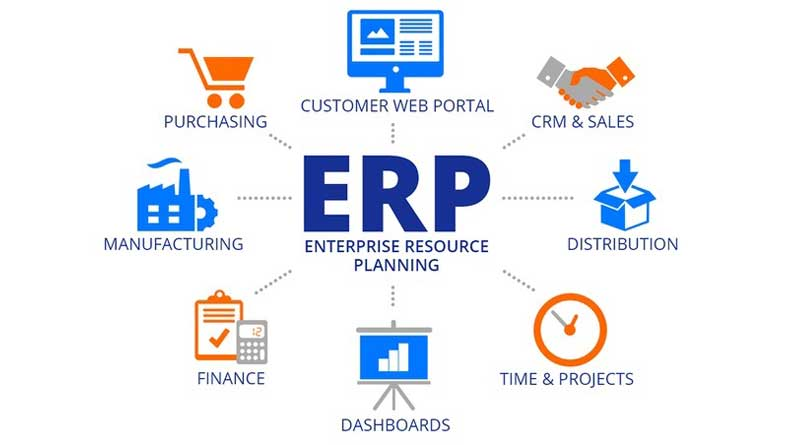
\includegraphics[width=\linewidth]{erp}
\end{center}


A company usually consists of multiple departments and each department has its own functions 
processes that are performed within the region of this department but there exist the integrated 
business processes that companies use to perform their work which cut across the departments. 
ERP provides a way to manage these integrated processes from beginning to end by facilitating information 
sharing and connection between these departments. \newline \newline


ERP systems usually group common Function areas into so-called business Module like\\

\begin{adjustwidth}{2cm}{}
\textbf{Financial management} This module manages your capital inflow and outflow. It covers standard Accounting \& Finance transactions like ledger, balance sheet, tax management, and payments. The module also generates financial reports for different departments and business units.\\\\
\textbf{CRM} This module helps you to boost customer service and, eventually, profit. It manages leads, opportunities, and customer issues. Likewise, it provides a 360-degree profile of your customers by consolidating data like their social media activities, purchase history, and past interactions with support reps.\\\\
\textbf{Sales \& Marketing} This module handles sales workflows like sales inquiries, quotations, sales orders, and sales invoices. The Sales and CRM modules work together to speed up the sales cycle and earn the company more profits.\\\\
\textbf{Manufacturing} This module is sometimes referred to as Engineering or Production. It helps businesses make manufacturing more efficient in areas, such as product planning, materials sourcing, daily production monitoring, and product forecasting.\\\\
\end{adjustwidth}

ERP job is to coordinate between the various systems that the business needs and make seamless integration with a shared database between them, hence eliminating common problems like

\begin{itemize}
    \item No real-time data access for other departments.
    \item Latency to get information.
    \item More than one department having a need for the same data will cause high cost as data maintenance will increase.
    \item Shared data will need to be synchronized or a department will think it’s lacking or having more than its needs.
    \item Moving information from one department to another is more prone to errors.
    \item Numerous disparate information systems are developed individually over time.
    \item Integrating date takes time and money.
    \item Inconsistency and Duplication of data.
    \item Lack of timely information leads to customer dissatisfaction and loss in revenue.
\end{itemize}

ERP usually offers its modules in a separate matter to give businesses the choice of the wanted modules they want integrate 
to eliminate the hassle of dealing with unwanted modules. When adding a new module it will also work with other existing added modules to perform 
integration with different modules.\\\\
The core component of an ERP system is the database as the integration can happen because of the shared database so it needs to be fast and responsive to perform well.\\\\

The dominant existent ERP systems are \textbf{SAP} and \textbf{Oracle ERP} they get most of the market shares besides \textbf{Odoo} which many organizations are moving their business to 
as it an open source ERP system who offers many features that the big two also offers.\\\\

The ERP have already existed for many years now, and now the world is shifting of how to modernize ERP systems 
and modern ERPs are now going to the cloud and business intelligence direction both to offer better optimization and automation and reduce ERP prices to suit different businesses.


%\begin{figure}
%    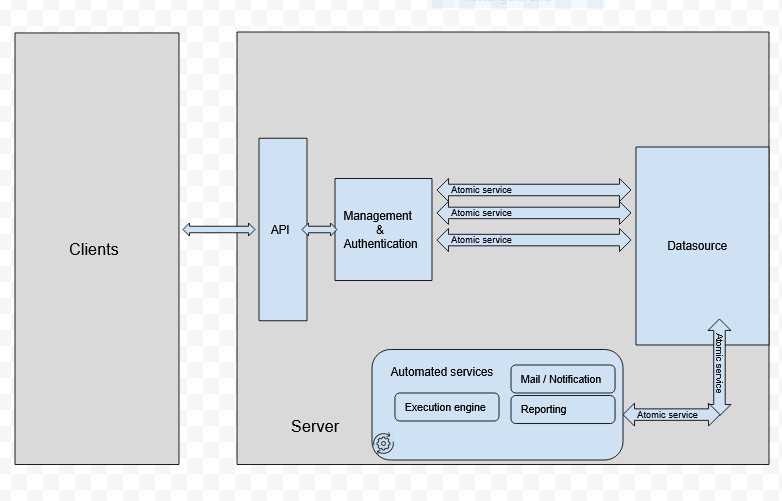
\includegraphics[width=\linewidth]{system_structure}
%    \caption{Test}
%    \label{fig:system_structure}
%\end{figure}


\chapter{The ERP}

The ERP is the name of our implementation of an ERP solution and using this name will always refer to our implementation.\\\\
The ERP has two main components
\begin{itemize}
    \item The main system which handles the system requests, controls the flow of data, and handles the users’ data.
    \item The system Modules that handle the business processes, We have a variety of modules to handle business needs.
\end{itemize}

\section{Main System}
Here we will talk about The ERP Features, Development, and internal structure and explore each component in the structure. Let’s begin with The features

\subsection{System Features}
The ERP is Open source, cross-platform, and cloud-based, so users can use it from homes, so no need for the companies using it to have huge buildings or offices to hold down their employees. This will help startups to push their businesses out without the need for huge financial support. Also, The ERP is multi-organizational, meaning that multiple organizations can use it at the same time. Finally, The ERP is very modular in design and can be expanded easily due to its modularity and simplicity.

\subsection{Development}
The ERP server and main functionality are written in C\# based on the brand new open source and cross-platform framework Asp.net core developed by Microsoft.\\\\
Modules services are written in C++ and compiled as DLL files and then gets loaded by the ERP when needed at runtime. Client-side is mostly written using Angular framework with some libraries like Bootstrap and JQuery. For Data storage we used Microsoft SQL server and MySQL database management systems and tools like swagger for API documentation. Next, you will find a table summarizing the tools used for development. Let’s talk a little bit about the main tools we use and why we chose them.
\\
\begin{adjustwidth}{2cm}{}
    \textbf{Asp.net core}\\
    %\begin{adjustwidth}{1cm}{}
        Is a cross-platform, open-source, high-performance framework for building 
      Cloud-based, Internet-connected applications. With ASP.NET Core, you can
      \begin{itemize}
        \item Build web apps and services, IoT apps, and mobile backends
        \item Use your favorite development tools on Windows, macOS, and Linux
        \item Deploy to the cloud or on-premises
        \item Run on .Net Core or .Net Framework
      \end{itemize}
    %\end{adjustwidth}
    \par\vspace {.5cm}
    \textbf{Why ?}\\
    %\begin{adjustwidth}{1cm}{}
        Before we list the reasons, we’d like to point out that the main goal or reason
      is learning new stuff and get the work done by this stuff\\
      This framework is not mature enough and there is not that much of a community using it to help us when we face problems but we accepted the challenge and went on with it
      \\\\
      Here are some of the main reasons
      \begin{itemize}
        \item It’s a redesign of Asp.net 4.x with architectural changes that result in a leaner and more modular framework
        \item Open-source
        \item Cross-platform
        \item Easy integration of the client-side framework
        \item MVC easily implemented
        \item Built-in dependency injection
        \item A lightweight, high-performance, and modular HTTP request pipeline
        \item Ability to host on IIS, Nginx, Apache, Docker, or self-host in your own process (Kestrel)
      \end{itemize}
    %\end{adjustwidth}
    \par\vspace {.5cm}
    \textbf{DLL}\\
    %\begin{adjustwidth}{1cm}{}
        Stands for Dynamic Link Library and it’s a Shared Library that can be used by more than one program at the same time and can be loaded into the program while running.
By wrapping each of The Erp Modules services in a DLL file, we can modularize our software and load them when needed only, this will help us save a lot of resources and enable us to have the ability to sell each module, maintain them and apply repairs, or upgrade to them separately and the system functions will not be affected.
\\\\
    %\end{adjustwidth}
\end{adjustwidth}


\subsection{Tools}

\begin{table}[h!]
\centering
\begin{tabular}{ |p{3cm}|p{3cm}|p{3cm}|p{3cm}|  }
    \hline
    \textbf{Tool} & \textbf{usage} & \textbf{Requirement} & \textbf{Programming language}\\
    \hline
    Asp.net core  & server and main functionality  & net core 2.2.x
    runtime
    Or SDK  & C\#\\
    \hline
    Angular  & Client-side development  & Node.js-8.12.0
    AngularCLI 7.3.8  & Typescript Javascript Html\&CSS\\
    \hline
    Entity framework
core & An ORM to deal with the
database & shipped with the
framework & C\#\\
    \hline
    DLL & Contain modules and main
    system services & C++ compiler & C++\\
    \hline
    MicrosoftSQL
server & Data Source to store
system data & MicrosoftSQL
server & SQL\\
    \hline
    MySql & Data Source to store
    system data & MySql & SQL\\
    \hline
\end{tabular}
\caption{summary of the ERP tools used for development}
\label{table:1}
\end{table}


\subsection{System Structure}

The main components of the system are shown in the fugure \ref{fig:system_structure} which will be explored in
detail in the coming sections

\begin{figure}
    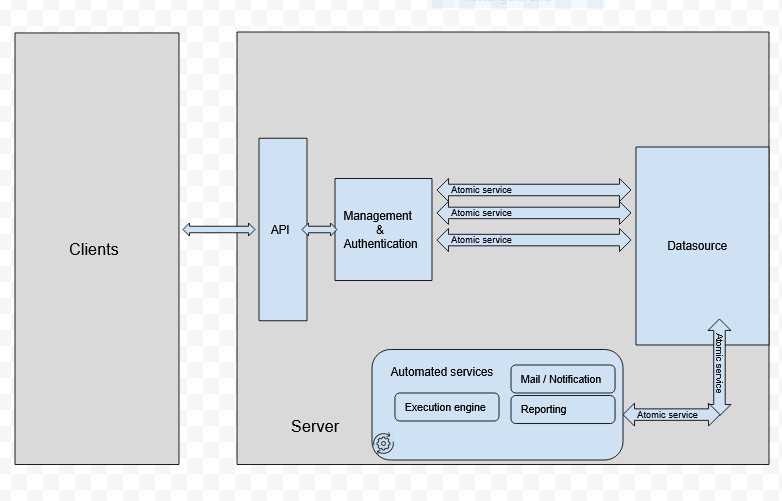
\includegraphics[scale=0.5, width=100mm]{system_structure}
    \centering
    \caption{ERP System Structure}
    \label{fig:system_structure}
\end{figure}


\subsubsection{System Main Components}

\begin{adjustwidth}{2cm}{}

    \textbf{API}\\
    %\begin{adjustwidth}{1cm}{}
        Stands for Application Programming Interface, is an interface that simplifies the access to
one’s application services from another application, so it’s the gateway to The ERP
Services.\\\\
For web-based API as in The ERP, each service will have a URL like \url{http://www.TheErp.com/app/GetProducts }, and in order to use this service an HTTP request will
be sent to this URL with some data (if required by the services), then the service gets invoked,
and then return the result in the form of HTTP response.\\\\
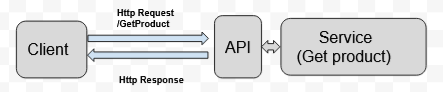
\includegraphics[width=100mm,scale=0.5]{system_api}\\\\
The ERP API is well documented using the swagger tool, so any external system that is
interested in using The Erp services can use this documentation.\\\\
    %\end{adjustwidth}

    \textbf{Role Management \& Authentication}\\
    %\begin{adjustwidth}{1cm}{}
        It is used to limit the access for certain services in The ERP.
        First, it Authenticates the incoming requests, in case of browser we use cookie
        Authentication; otherwise, Jwt Authentication is used, after authentication we can find out
        some info about the invoker like username, user id, roles (Administrator, manager, ..etc), and
        company name because like we said before, The ERP can be used by multiple organizations
        at the same time, so the company must be included. The reason why we can find this info, is
        after a login request from a client has been validated, this info gets encrypted as a cookie in
        case of a client browser or a token otherwise, and sent back with the HTTP response to the
        login request, so that when a client calls a service which requires Authentication, the client
        must include the cookie or the token it received after successfully logged it in the HTTP
        request and then it gets decrypted and the information can be deduced.\\\\
    %\end{adjustwidth}

    \textbf{Services}\\
    %\begin{adjustwidth}{1cm}{}
        First of all, let’s define the term service. A service, in the case of The ERP, is a job that we
want The ERP to do it for us, like getting an order, sending an email, or giving a report of the
financial situation ..etc.
If we look deeper into these jobs we can find out that some of them can be divided into
smaller jobs. For example, getting an order, it first checks that the products in the order are in
stock then accepts the payment, if they are, then send the order; otherwise, orders the
manufacturing to start to produce this product and inform the customer.
These smaller jobs are called, in our system, Atomic services because they can’t be divided
into smaller jobs.\\
These Atomic services can be used as a building block for other big services, such as in the
case of sending an order. And it can be used as a service itself. So the bottom line is that The
Erp is only containing services that are atomic in nature.
Above that, the services are a composite of these Atomic services.\\\\
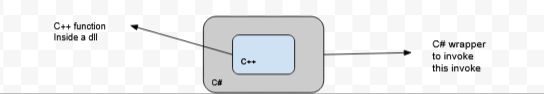
\includegraphics[width=100mm,scale=0.5]{atomic_service}\\\\
If we zoom in on atomic services we will find out that they consist of C++ functions and C\#
wrapper to serve as an interface to the C++ code.\\
Another kind of the services The ERP provides is the Automated Services .
Automated services are the kind of services that run on their own, they do not need an invoker
to run and The ERP is filled with them, below we list the important ones and their jobs\\
\linebreak
\begin{itemize}
    \item \textbf{Real-Time Data}\\ This automated service is continuously monitoring the database for changes and if there is
    any, it will update the users with these changes to keep the data they have intact.\\
    \item \textbf{Notification System}\\ It’s connected to all active users. Continuously sending notifications to them about their
    assigned Task, monitor the database for unsent emails then sent them.\\
    \item \textbf{Reporting}\\ Its job is to produce reports. For example, in case of a problem (connection to the database
    server or the manufacturing machines failed,.... ) it will try to contact any of the
    administrators by sending an email or an SMS to notify them about the problem to deal with
    it.\\
    \item \textbf{Execution Engine Fig \ref{fig:poll}}\\
    
\end{itemize}

\begin{figure}
    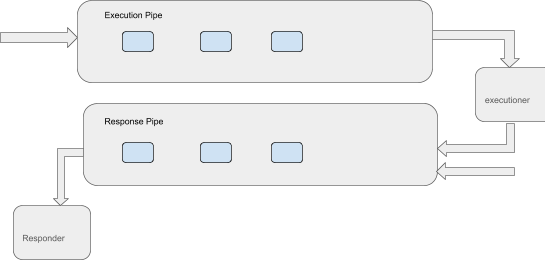
\includegraphics[scale=0.5, width=100mm]{poll}
    \centering
    \caption{Execution Pipe}
    \label{fig:poll}
\end{figure}

    %\end{adjustwidth}

    \textbf{Execution Engine}\\
    %\begin{adjustwidth}{1cm}{}
        It consists of two pipes (Execution and Response). A task is put into the execution pipe then
pulled by the executioner to be executed. If a problem occurs (failed to connect to the
database server) during execution, the executioner will then put the task back in the execution
pipe for another trail.\\
If the execution produces a result, like for example (GetCustomer), it will be put into the
response pipe to be sent back to the invoker of the Task and so on.\\
This helps when a problem led to make the services requests through API call unable to be
invoked. For example, failed to connect to the data source, so the solution is instead of
invoking them when requested through the API, which will lead to failure, we put them into
the Execution Queue and we know the rest.\\
Another big use is when the service requested through the API is not atomic or it’s atomic but
Time-consuming, in that case, the services can be put one by one into the execution pipe and
it will be taken care of. This will make the system more responsive.
    %\end{adjustwidth}
        
        
    
    
\end{adjustwidth}

\section{The Modules}

The modules are interconnected with each other and often have jobs to that each will have a share in
like and they are integrated using the ERP.\\
The modules can be added separately to give users the customization and the choice of their business
needs without overwhelming them with unneeded modules.\\
Our modules including, but not limited to, as we are working on new modules
\begin{itemize}
    \item CRM
    \item Warehouse Management
    \item Accounting
    \item Manufacturing
\end{itemize}

\break
\subsection{CRM}
CRM (Customer Relationship Management) is a strategy to manage the relationships of the company.
It makes communicating with customers easier and improves marketing.
\begin{center}
    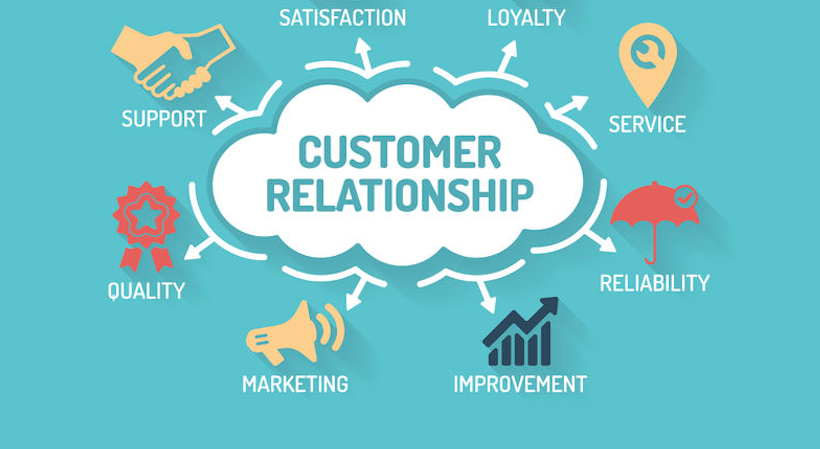
\includegraphics[width=\linewidth]{crm}
\end{center}

%\begin{figure}
%    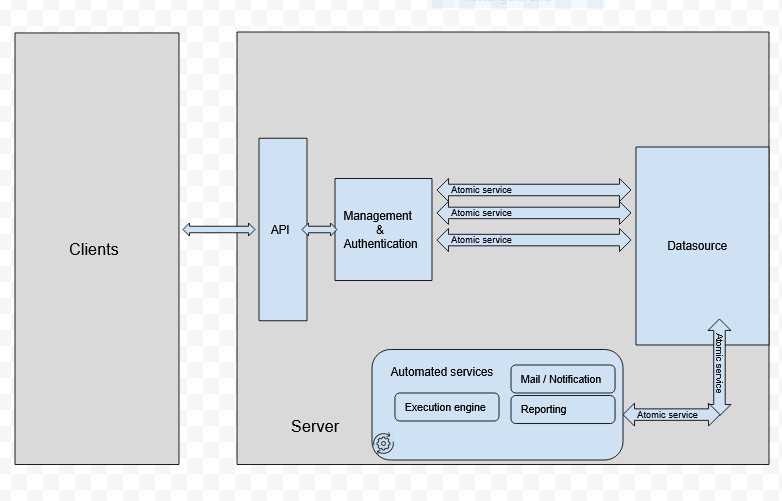
\includegraphics[width=\linewidth]{system_structure}
%    \caption{Test}
%    \label{fig:system_structure}
%\end{figure}
\subsubsection{Main features of CRM}
\begin{itemize}
    \item Customer Management
    \item Sales Management
    \item Reporting
\end{itemize}
\subsubsection{Customer Management}
We collect and manage customer information and their interests.
\begin{itemize}
    \item Qualified customers (Who have made orders)
    \item Non-Qualified customers (Who are considered to be the lead or target of the sales team)
\end{itemize}
Sales team communicates with non-qualified customers to make deals according to their interests of
products.\\
If the customer accepts the deal, an opportunity, that has some products of customer’s interests, is
created.
\subsubsection{Sales management}
We manage the sales through a pipeline of opportunities, each opportunity goes through 5 main stages
which are (New, Qualified, Proposition, Negotiation, and Won).\\
When an opportunity is created, it is in New stage, then a salesperson communicates with the
customer to make a deal with them. If the customer accepts the deal, the opportunity will be changed
to Qualified.\\\\
After that, a salesperson proposes some products that the customer has an interest in and negotiates
about their price. If the customer accepts to buy this product, the opportunity will be changed to Won
and will be created as an order in the system’s database.
\subsubsection{Reporting}
With CRM, salespeople and managers have access to dashboards where they can easily view
important opportunity KPIs, in the form of graphs, charts, and more. They can also export data and
create reports. This allows employees to analyze opportunities, and thus gain insights into sales and
marketing activities. You can also analyze lost/won opportunities to improve your conversion rates.
\newpage

%\begin{figure}
%    \centering
%    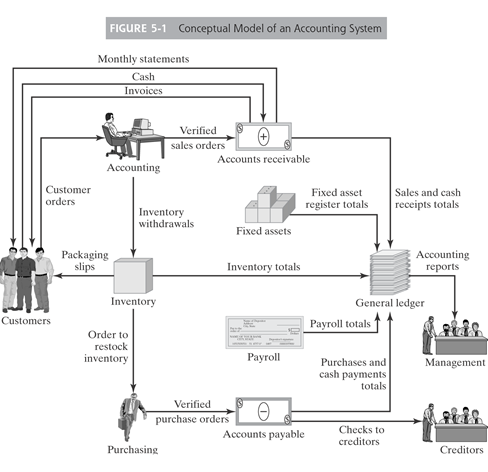
\includegraphics[width=\linewidth]{crm_workflow}
%   \caption{CRM Workflow}
%    \label{fig:crm_workflow}
%\end{figure}

\subsection{Warehouse management}
Warehouse management refers to the various processes related to maintaining and controlling a
business’ warehouse, such as the shipping, receiving, put-away and picking of goods. Warehouse
management is responsible for everything that happens in a warehouse, whether they own one
warehouse or several.\\\\
Managing inventory in warehouses with pen and paper can be inaccurate, slow and a lot of work,
that’s why it’s better to use a Warehouse management system.

\begin{center}
    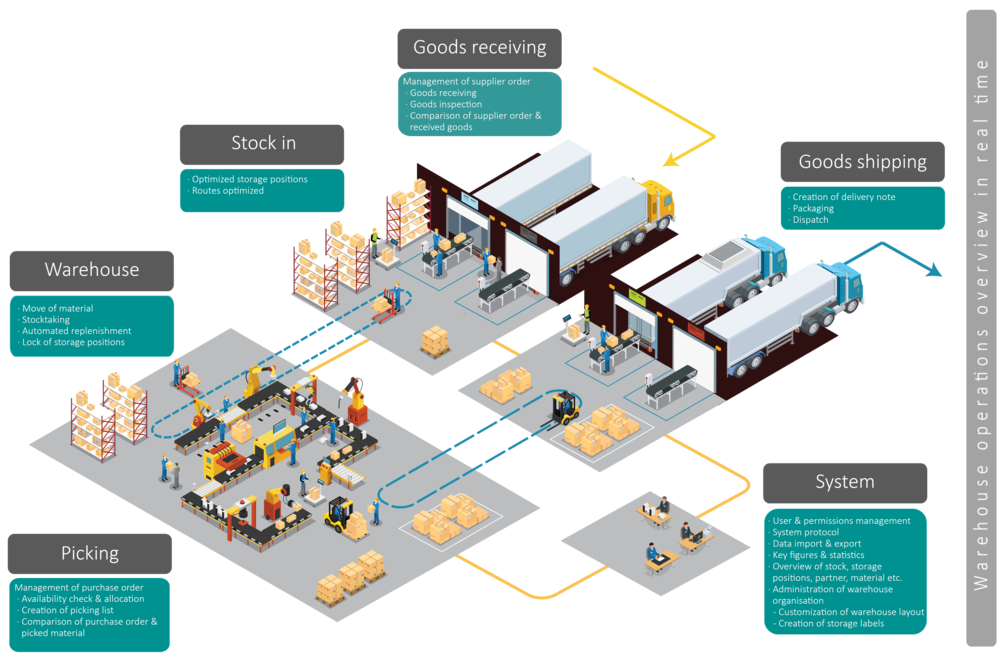
\includegraphics[width=\linewidth]{wms}
\end{center}

\subsubsection{Warehouse management system}
Warehouse management system (WMS) is a piece of software that controls, records and automates
various warehouse operations. The goal is to increase the overall productivity and efficiency of a
business’ warehousing operations.
\subsubsection{What about our implementation of WMS ?}
Our WMS can be used as a standalone system or can be integrated into The ERP. It supports multiple
inventories, keeps track of products’ moves, provides constant reports about orders delivery time, and
has many other features.
\subsubsection{Features}
Uses a database configured to support warehouse operations, containing details describing a
variety of standard warehouse elements including
\begin{itemize}
    \item Individual items that are handled and stored using weight, dimensions, automatic ID
    labels (bar codes, etc.), number of units in inventory, location in inventory, and
    whether it’s sold or purchased
    \item Warehouse storage location and size
    \item Orders that are handled using automatic order number, customer’s information,
    payment details, and time and date details (order being made, order ready for
    shipping, and order delivery to the customer)
    \item Ordered items with their quantities
    \item Supply requests with their time and date, suppliers’ information, and the number of
    units to be supplied
\end{itemize}
Is responsible for
\begin{itemize}
    \item providing Status of item quantity in terms of in stock, ordered, and ready for shipping
    quantities
    \item Handling Multiple warehouses
    \item Following up with each order throughout its stages from being made until it’s ready
    for shipping
    \item Keeping track of products going in and/or out of inventories
    \item Organizing - sequencing the orders to be picked
    \item Reporting, which helps analyze the performance of warehouse operations, and find
    areas to improve
    \item Asking for supply when an item is out of stock
    \item Sending notifications when an order is completed
\end{itemize}
\subsubsection{Benefits}
\begin{itemize}
    \item Track locations, transaction histories, and costing
    \item Speed up the process of getting products into and out of inventory by keeping records of the
    location of each product inside the inventory
    \item Organizing - sequencing the orders to be picked helps Minimize the need for dock staging
    space, by having orders arrive at the shipping dock in trailer load sequence
    \item Proper reporting mechanism of inventory helps the manufacturing department in planning
    their future production schedules accordingly
    \item It helps track the payments and flow of finances into your Accounts
\end{itemize}
\newpage

%\begin{figure}
%    \centering
%    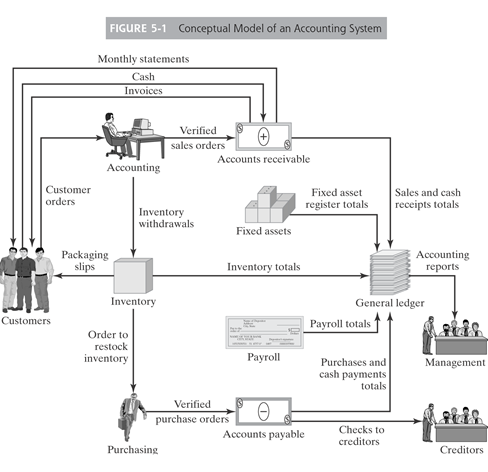
\includegraphics[width=\linewidth]{wms_workflow}
%   \caption{WMS Workflow}
%    \label{fig:wms_workflow}
%\end{figure}

\subsection{Accounting}
\begin{center}
    
\includegraphics[width=\linewidth]{accounting}
\end{center}
\subsubsection{Why Accounting ?}
The financial module in ERP Systems provides financial functionality and analysis reports for balance
sheets, ledgers, and financial statements.\\\\
Financial module is essential for an organization. Other modules cannot function without it.
Successful implementation of financials is highly required for an organization in order to be trusted.
All these factors explain the fact that financial modules are taken up first.\\\\
The finance module of an ERP system has the following sub-systems.
\subsubsection{Accounting Subsystems}

\begin{adjustwidth}{2cm}{}
\textbf{Financial Accounting}
    \begin{adjustwidth}{1cm}{}
        The objective of a good Financial accounting system is to provide control and integration
of financial information that is essential to strategic decision making. The Financial
accounting module of an ERP System gives you the ability to track financial accounting
data within an international framework of multiple companies, currencies, and charts of
accounts.\\
    \end{adjustwidth}
\textbf{General Ledger}
    \begin{adjustwidth}{1cm}{}
        General Ledger is essential to both, the financial accounting system and strategic decision
making\\
    \end{adjustwidth}
\textbf{Accounts Receivables}
    \begin{adjustwidth}{1cm}{}
        The Accounts Receivable Modules helps in tracking all the invoices that are awaiting
payment from customers\\
    \end{adjustwidth}
\textbf{Account Payable}
    \begin{adjustwidth}{1cm}{}
        Accounts Payable Module (AP) — provides the functionality to enter, monitor, maintain,
and process for payment of invoices and credit notes that the organization received from its
vendors\\
    \end{adjustwidth}
\textbf{Asset Accounting}
    \begin{adjustwidth}{1cm}{}
        \begin{itemize}
            \item Fixed asset management like acquisition, depreciation, retirement, etc
            \item Legal consolidation
        \end{itemize}
        A Legal consolidation process is a financial process that allows showing the assets,
financial position, and income of a group as if the group were a single enterprise\\
    \end{adjustwidth}
\textbf{Controlling}
    \begin{adjustwidth}{1cm}{}
        Controlling enables the possibility to plan the financial parameters of the company and
offers both, proactive capabilities for early warning if they become negative and complex
analysis tools to identify factors of influence\\
    \end{adjustwidth}
\end{adjustwidth}
\subsubsection{Accounting Processes}
\begin{adjustwidth}{2cm}{}

    \textbf{Budgeting}
        \begin{adjustwidth}{1cm}{}
            Analysis of allocations, expenditures, revenues\\
        \end{adjustwidth}
    \textbf{Cash management}
        \begin{adjustwidth}{1cm}{}
            Cash flow analysis\\
            What-if analysis\\\\\\
        \end{adjustwidth}
    \textbf{Capital budgeting}
        \begin{adjustwidth}{1cm}{}
            Evaluation tools: NPV, IRR, pay-back period\\
        \end{adjustwidth}

\end{adjustwidth}
\subsubsection{Our Module Features}
\begin{itemize}
    \item Show Company Accounting data
    \begin{itemize}
        \item Show Sales (The products sold and how much the company earned)
        \item Show Bills (Show the bills that the company has to pay and how much money is it)
        \item Show Payments (Show the payments the company made, buying products materials
        or paid for bills)
        \item Show Company invoices (For the payments have been made, if there was any)
    \end{itemize}
    \item Show Customers Accounting Data
    \begin{itemize}
        \item Billing data (Show the bills that the customer has to pay for the company)
        \item Invoices data (Show the customer’s invoice for each payment for the order he has
        made)
    \end{itemize}
    \item Show Real-time data
    \begin{itemize}
        \item To show data as soon as it changes with no need to refresh the page
    \end{itemize}
    \item Reporting
    \begin{itemize}
        \item Reports about profits, losses, and balance sheets
    \end{itemize}
    
\end{itemize}

%\begin{figure}
%    \centering
%    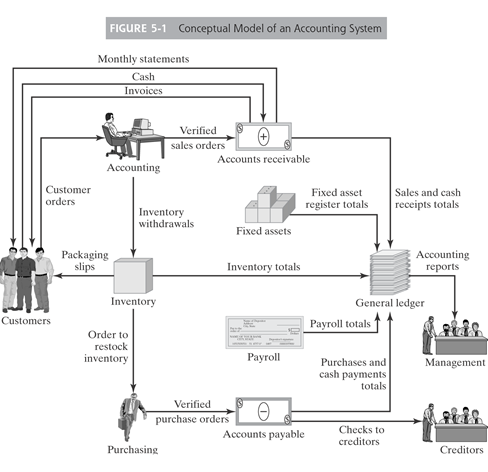
\includegraphics[width=\linewidth]{accounting_workflow}
%   \caption{Accounting Workflow}
%    \label{fig:accounting_workflow}
%\end{figure}

\break

\subsection{Manufacturing}
\begin{center}
    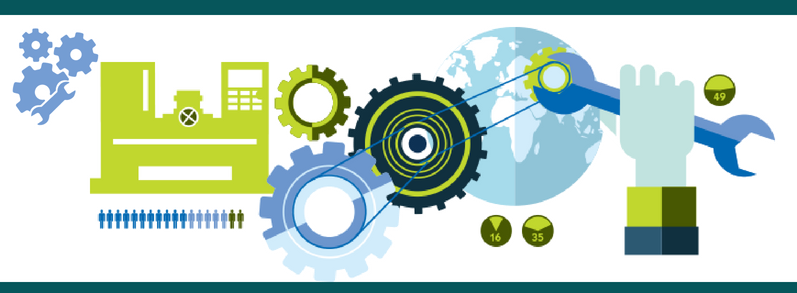
\includegraphics[width=\linewidth]{manufacturing}
\end{center}

In order to sustain in the stiff competitive market, manufacturing companies invest a lot of time
managing their diverse business functions rather than focusing on core business. This eventually leads
to less productivity and profitability in the business sector.\\
A manufacturing management software comes with an ample number of features that helps in
streamlining business operations, effectively transacting information across all business sectors,
ultimately focusing on enhancing the business workflows.\\
Manufacturing is the process by which raw materials are transformed into finished products.

\subsubsection{Manufacturing Module}
The role of ERP manufacturing module is to complete the inventory management by implementing
the operations specific to a streamlined manufacturing process. For a company, which handles a large
number of manufacturing products, they need to track every manufacturing order efficiently and
effectively.

\subsubsection{Our implementation of Manufacturing Module}
The Manufacturing Module in our system is independent and robust in handling the complexity of
Production, managing bills of materials, planning the manufacturing Orders, etc. Manufacturing
module is one of the basic applications in our system. Since the Manufacturing module is highly
integrated with Inventory Management, you can keep your inventory automatically updated with each
manufacturing process.\\
Our implementation of the manufacturing module helps businesses by dealing with the following
subjects
\subsubsection{Products}
Manufacturing module gives you the ability to add your manufacturing end products and determine a
bill of materials for each product by using a friendly user interface.
\subsubsection{Bill of materials}
Bill of Materials (BoM) is the basic building block of any manufacturing process. It is the list of raw
material needed to produce a product. So while creating a manufacturing order for a particular
product, one needs to select corresponding BoM. BoM will help the user to keep the inventory
updated during the manufacturing process.\\
BoM allows a flexible environment for custom builds without starting from scratch.
\subsubsection{Manage Production}
Once you have created and confirmed a Manufacturing order, you can start production. Our system
will list all the Manufacturing orders.\\
After making your order, our manufacturing system will place your orders in a list describing the
status of your order according to the inventory management system, starting date, and the current state
of your order (done, canceled, confirmed).
\subsubsection{Robust Inventory Tracking}
Manufacturing plants deal with raw material and finished goods inventory. Raw material management
is the process of keeping track of all appropriate material required to ensure that the business carries
on uninterrupted manufacturing processes. On the other hand, finished goods inventory includes
products that the manufacturing plant has produced, and they need to be managed to keep track of
how and when they would be transported to the warehouses or customers.\\
This is where many manufacturing modules experience challenges, as these two processes must be
synchronized to avoid inappropriate or insufficient production, which would bring customer
dissatisfaction, and cause losses to the business.\\
Keeping watch on these manually is quite impossible. For this, you need an ERP software that can
track complete inventory. The automated application would help reduce human errors and improve
inventory management like raw materials re-ordered needs or track the delivery dates of the finished
goods, etc., thus keeping your manufacturing running seamlessly.\\
From that context, our manufacturing system has a robust inventory tracking since you have placed
your order and in case of lacking raw materials, manufacturing module will change the status of your
order to waiting, until the raw materials are available. Our manufacturing module will track these
changes and update your order status.

\subsubsection{IOT Box}
IOT Box is one of the important features that our system offers, As it provides a way for the system to
communicate with hardware components directly. This will give the business even more managing
capabilities by integrating the hardware in the system to monitor the hardware and the process it does.\\
IOT box is a physical box that we offer that can be connected to our system directly and the box can
be then connected to the business hardware, like physical machines, to do its job.\\
The current IOT box is limited in features as it will send commands to the box that can in return send
them to the hardware we want to control. It works as a microcontroller that can be programmed from
the system to do its functions.\\
The IOT box is tended to have more capabilities and have different ports added to it to be used for
different activities.

%\begin{figure}
%    \centering
%    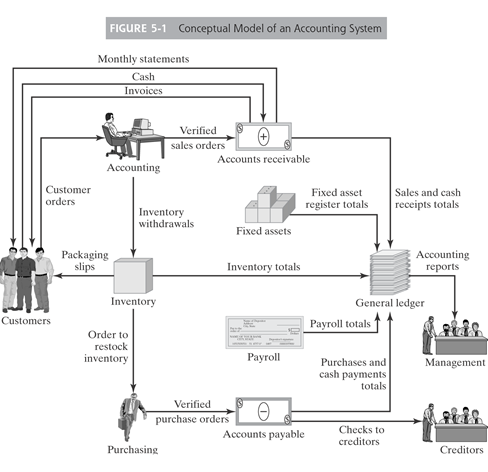
\includegraphics[width=\linewidth]{manufacturing_workflow}
%   \caption{Manufacturing Workflow}
%    \label{fig:manufacturing_workflow}
%\end{figure}

\break
\subsection{Product Manager}

\begin{center}
    
\includegraphics[width=\linewidth]{product}
\end{center}

Product manager refers to a way to show the products and offers a way to sell the products for businesses that want to sell their products.
\subsubsection{Our Product Manager}
\begin{itemize}
    \item Offers a page that can be shown to customers with a specific Link
    \item A system to add customers to log in and out of the system
    \item A way to add the products to cart and buy them
\end{itemize}
This help businesses to control their selling products page from inside the system which is the goal of our solution of having one system to control them all.\\\\


\chapter{System Access}

\section{The ERP}
We wanted to achieve, with The ERP, the ability for the users to be able to use the system from
anywhere to give the users more diversity of the places they can check the system from or achieve
tasks and also give the users the ability to determine what can be achieved and from where to satisfy
business rules and security.\\\\

\begin{center}
    
\includegraphics[width=\linewidth]{cloud}
\end{center}

To achieve this. The ERP comes with more than one plan, the first is to have the code for the program
and use it within the company.\\\\
To achieve the more diversity options, The ERP will be on the cloud for different businesses to use
and benefit from it, which allows users to access it from anywhere and also with a mobile app to have
a more concise view of the system.

\section{Mobile Application}
\subsection{ERP App Main Task}
The main task of the ERP app is to provide an easy way to monitor the modules of the ERP system
\subsection{Main Features}
\begin{itemize}
    \item Authenticate admins
    \item Authenticate users
    \item Rest API with the main ERP server
    \item Display all modules
    \item Display statistics of each module
\end{itemize}

\subsection{Application Screens}
\begin{itemize}
    \item \textbf{Authentication sign up screen}\\ Responsible for registering the full data needed of the customer or the admin of the
    module.
    \item \textbf{Authentication login screen}\\ Responsible for getting email and password from the user for authentication.
    Get the user type if admin or customer.
    \item \textbf{Modules Screen}\\ Displays all modules
    \item \textbf{CRM Screen}\\ Displays more information about the module and some statistics about the customers
    \item \textbf{Billing \& Accounting Screen}\\ Displays more information about the module and some statistics
    \item \textbf{Warehouse Management Screen}\\ Displays more information about the module and some statistics
    \item \textbf{Profile Screen}\\ Displays the current modules and some settings of the application

\end{itemize}

The ERP application is made with flutter which is Google’s mobile app SDK, complete with a
framework, widgets, and tools, that gives developers an easy way to build and deploy visually
attractive, fast mobile apps on both Android and iOS platforms.


    \part{BPM}
    \chapter{Introdution}

With this new part, we will get to discover a new way to approach business processes and help
improve our business, it has its own unique way that is different from ERP approach but to get BPM
approach we will need to understand what a business process is.\\\\
A business process is an activity or set of activities that can accomplish a specific organizational goal.
Business processes should have purposeful goals, be as specific as possible, and have consistent
outcomes. It is a collection of activities that takes one or more kinds of input and creates an output,
such as a report or forecast, that is of value to the customer.\\\\
ERP software supports executing business processes by supporting the efficient operation of business
processes by integrating tasks related to sales, marketing, manufacturing, logistics, accounting, and
staffing—throughout a business. In addition to this cross-functional integration, which is at the heart
of an ERP system, companies connect their ERP systems, using various methods, to coordinate
business processes with their customers and suppliers.\\\\
So how does BPM come in the picture? Business Process Management (BPM) is an approach that
focuses on capturing and improving business processes to make an organization more efficient. This
can be achieved by first capturing an organizations’ current-state end-to-end processes and then
documenting the steps in process maps.\\\\
While the ERP job cares more about cross-functional integration and tends to be limited to
organizational functions, BPM job tends to be much more process-focused.\\\\
Most companies, when undertaking a business improvement initiative, will consider implementing a
dedicated BPM system to help them model, analyze, and optimize processes to drive the business
transformation forward.\\\\
BPM tends to be flexible with approaching business processes design. It can manipulate, change, fix
and monitor a business process easily. The usual cycle of BPM fig \ref{fig:bpm_flow} helps to achieve this
flexibility which includes
\begin{figure}[h]
    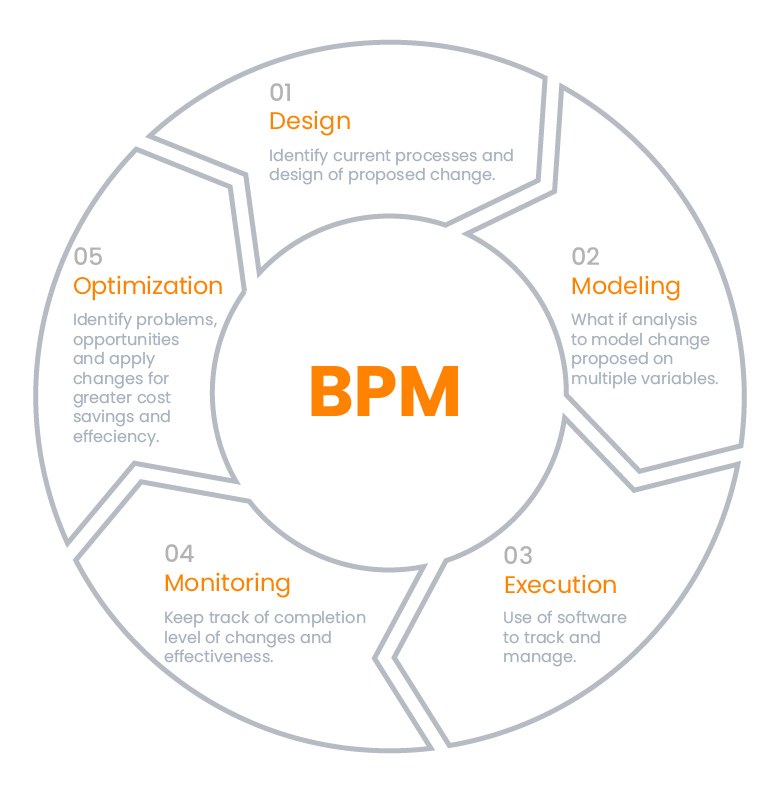
\includegraphics[width=80mm]{bpm_flow}
    \centering
    \caption{BPM Cycle}
    \label{fig:bpm_flow}
\end{figure}
\begin{itemize}
    \item \textbf{Design} Process design encompasses both the identification of existing processes and the
    design of future processes. Areas of focus include representation of the process flow, the
    factors within it, alerts and notifications, escalations, standard operating procedures, service
    level agreements, and task hand-over mechanisms
    \item \textbf{Modeling} Modeling takes theoretical design and introduces combinations of variables. For
    example, changes in rent or materials costs, which determine how the process might operate
    under different circumstances.
    \item \textbf{Monitoring} Monitoring encompasses the tracking of individual processes, so that
    information on their side can be easily seen, and the status of their performance of one or
    more processes can be provided. In addition, this information can be used to work with
    customers and suppliers to improve their connected processes and measures information of
    three categories: cycle time, defect rate, and productivity
    \item \textbf{Optimization} Process optimization includes retrieving process performance information
    from modeling or monitoring phase; identifying the potential or actual bottlenecks and the
    potential opportunities for cost savings or other improvements; and then, applying those
    enhancements in the design of the process. Process mining tools are able to discover critical
    activities and bottlenecks, creating greater business value
    
\end{itemize}



We mentioned that BPM helps capture end-to-end processes, but \textbf{what does end-to-end process really
mean}\\\\
What end-to-end process really means is from start to finish. The goal is to understand and thus to assess and improve an entire process —not just its components.
\\

\section{What is a process ?}
A process is a sequence of tasks. Every task is an action, and is carried out by a person
or by some automatic system. All processes share certain characteristics, The characteristics were referenced from the book 
Designing Efficient BPM Applications \cite{bpmapp} and was the basis of how we had chosen our notation for modeling\\

\textbf{\textit{Interaction over time}}
\begin{adjustwidth}{2cm}{}
    A chronological relationship between tasks, with due dates and sequencing but
not a schedule.\\
\end{adjustwidth}
\textbf{\textit{Multiple actors}}
\begin{adjustwidth}{2cm}{}
    More than one person or automatic system must complete tasks for the whole
process to be successful.\\
\end{adjustwidth}
\textbf{\textit{Repetition}}
\begin{adjustwidth}{2cm}{}
    The sequence of tasks is repeated, either at fixed intervals or when triggered by a
specific event.
\end{adjustwidth}

\section{What Is Not a Process ?}
The action of filling out a form is not a process. A form that has many pages and is
filled out online is a single task for a single user. A form that can be filled out in more
than one sitting is a single task for a single user. Even a form that has smart fields that
depend on other fields, with conditional display, is a single task for a single user.
A state diagram is not a process. A process is constructed from actions. The things
that are updated by these actions might have states associated with them, so you
might create state diagrams as part of your process validation, but the state diagram is
not itself a process.

\chapter{The BPM}

Yet again we have a name for our implementation of BPM that we will use over the next few chapters
and it follows the same pattern for our naming schemes, \textbf{“The BPM”}.\\\\
The BPM is meant to work best when integrated with other applications to be used to its potential. It
will provide all the tools to be used inside other programs. But it still works as a full Standalone BPM
solution to design, execute and monitor Business processes.\\\\
It offers a pipeline that works on three stages each can work as a standalone application, the pipeline
works as follows
\begin{itemize}
    \item Design business process using a graphical application
    \item Execute the business process with the ability to modify its execution at runtime
    \item Monitor the business process and see the process execution in detail and change the execution
    graphically
\end{itemize}

\section{The Process}

For each process The starting conditions and timetable of a process. The following question need to be considered\\\\
Under what conditions will the process start ? These conditions were referenced from the book Process-Driven Applications \cite{processbpmn}\\
\begin{itemize}
    \item \textbf{Time}\\
    The process starts at a particular time\\
    The process starts after a particular time interval\\
    The process starts in relation to another time\\
    \item \textbf{Conditions}\\
    The process starts once one or more conditions are met, for example, a
    warehouse is restocked with a particular product once stock levels go
    below a predefined threshold value.
    \item \textbf{Messages}\\
    The process waits for a particular message to arrive.
    \item \textbf{Events}\\
    Events have an important role, especially in exception situations. An event
is triggered when an extraordinary situation arises that requires special handling, for example, a late delivery, a machine failure, an accident, or Similar.
\end{itemize}

After the designer answers these questions, he will change the setting of the starting node to satisfy
the conditions required for this process.\\\\
For each process, there will be three start nodes, two of which will have their starting conditions
embedded in them
\begin{itemize}
    \item The first will be triggered when the process loaded in the engine can be used to
    initialize data related to the process or when integrated with a GUI application that
    can be used to generate a GUI for the process when loaded.
    \item The second will be when the process awakes and starts to run, whether it is its first
    time to run or awaken after a pause, can be used to get data to memory back before
    continuing the process.
    \item The third will be the one which will start based on the question that the user answered
    and can choose which event will make it start.
   \end{itemize}

\subsection{Involved Process Roles}
The involved process roles define who is responsible for performing which
activities during the process. All you need is a simple list of process roles and a
description of the functions the roles perform within the process. At runtime, users
and groups from the company’s user management solution are assigned to these
roles. Although this presents a challenge, the complex task of assigning users to
process roles in workflow management systems within company organizations is
outside the scope of this book and is not discussed in more detail here.

\section{Notation}
While designing our notation we came across two other notations that are used as standards like\\\\

\textbf{BPMN 2.0} \cite{OMG-BPMN} (Business Process Model and Notation), it provides
businesses with the capability of understanding their internal business procedures in a graphical
notation and will give organizations the ability to communicate these procedures in a standard
manner.\\\\
\textbf{BPEL} \cite{OASIS-BPEL} (Business Process Execution Language) is an XML based language that allows Web services
in a service-oriented architecture (SOA) to interconnect and share data.\\\\
Our notation is affected deeply by BPMN 2.0, but our goal was simplicity so we removed some of its
complexity and added some other nodes that can be used in an easy and intuitive manner, So while
BPMN 2.0 is much capable of executing complex business processes. Our notation is much more
simpler to use and understand.

\subsection{The Nodes}
They should be descriptive enough to understand business process like interaction with users and
repetition of tasks, simple to be intuitive to use and have the ability to be extended for advanced
usage. \\\\

\large \textbf{Start}\\

\begin{tabular}{C{2.2cm}  L{10cm}}
    
\includegraphics[width=\linewidth]{start} & Specifies the start of the flow.\newline 
    Each flow will have start nodes that will have trigger events\newline
\end{tabular}

\break

\large \textbf{End}\\

\begin{tabular}{C{2.2cm}  L{10cm}}
    
\includegraphics[width=\linewidth]{end} & Specifies the end a branch flow.
    \newline Each flow can have one or more than one end node.
    \newline Each will be the end of one flow or more than one.

\end{tabular}

\par\vspace {1cm}

\large \textbf{Service Task}\\

\begin{tabular}{C{2.2cm}  L{10cm}}
    
\includegraphics[width=\linewidth]{task} & Executes Web services based on REST.
    \linebreak Will Create the request and handle the response.

\end{tabular}

\par\vspace {1cm}

\large \textbf{Database}\\

\begin{tabular}{C{2.2cm}  L{10cm}}
    
\includegraphics[width=\linewidth]{database} & connects with a SQL database and send sql commands to it.
    \linebreak Can listen to the database for data insertion using polling.

\end{tabular}

\par\vspace {1cm}

\large \textbf{Parallel}\\

\begin{tabular}{C{2.2cm}  L{10cm}}
    
\includegraphics[width=\linewidth]{parallel} & Makes more than one flow to be executed in the same process.
    \linebreak The two flows will be executed at the same time.

\end{tabular}

\par\vspace {1cm}

\large \textbf{Condition}\\

\begin{tabular}{C{2.2cm}  L{10cm}}
    
\includegraphics[width=\linewidth]{condition} & Divides the flow into more than one flow, each with a condition.
    
\end{tabular}

\par\vspace {1cm}

\large \textbf{External Event}\\

\begin{tabular}{C{2.2cm}  L{10cm}}
    
\includegraphics[width=\linewidth]{task} &Executes Events from outside of The BPM nodes.

\end{tabular}

\par\vspace {1cm}

\large \textbf{Timer Event}\\

\begin{tabular}{C{2.2cm}  L{10cm}}
    
\includegraphics[width=\linewidth]{timer} &Waits for a certain time before proceeding with the flow.
\end{tabular}

\par\vspace {1cm}

\large \textbf{Script}\\

\begin{tabular}{C{2.2cm}  L{10cm}}
    
\includegraphics[width=\linewidth]{script} &Executes a predefined script written by user to add functionality to The
    BPM.
\end{tabular}

\par\vspace {1cm}

\large \textbf{Json}\\

\begin{tabular}{C{2.2cm}  L{10cm}}
    
\includegraphics[width=\linewidth]{json} &Creates a JSON string or get the values of the elements in a java string.
\end{tabular}

\par\vspace {1cm}

\large \textbf{Increment Function}\\

\begin{tabular}{C{2.2cm}  L{10cm}}
    
\includegraphics[width=\linewidth]{add} &A function that increase variable by 1 used in loops
\end{tabular}


\section{Tasks}

Tasks are the main components of The BPM. Each business process will have a variety of tasks that
need to be executed. The BPM supports different kinds of tasks.

\begin{itemize}
    \item \textbf{API Tasks} \\
    They are tasks that are defined through an API which is a defined interface of how to interact
    with other applications functions. It can be used to add functionality to The BPM by
    executing functions available at other places
    \item \textbf{Script Tasks} \\
    They are tasks that are defined through an API which is a defined interface of how to interact
    with other applications functions. It can be used to add functionality to The BPM by
    executing functions available at other places
    \item \textbf{User Tasks} \\
    A User Task is used to model work that needs to be done by a human actor like filling a form
or accepting a request.

\begin{figure}[h]
    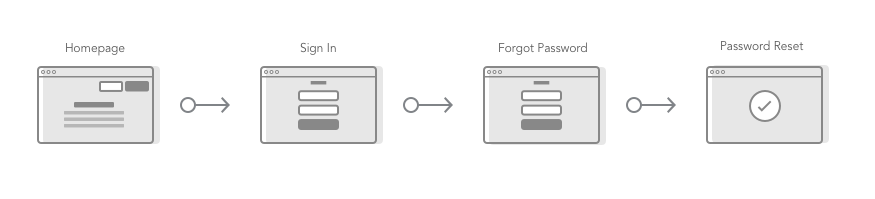
\includegraphics[width=\linewidth]{user_task}
    \centering
    \caption{User Task}
    \label{fig:user_task}
\end{figure}

    \item \textbf{External Tasks} \\
    They are tasks that are only known to the business, and they have no defined way of accessing
them from outside of the system, so the only way to execute them is by executing them inside
of the system, So The BPM will define a way to define the tasks by the names known to the
business and will put them in a Queue waiting for the system to look for them and get them
then execute them. Fig \ref{fig:task_worker}

\begin{figure}[h]
    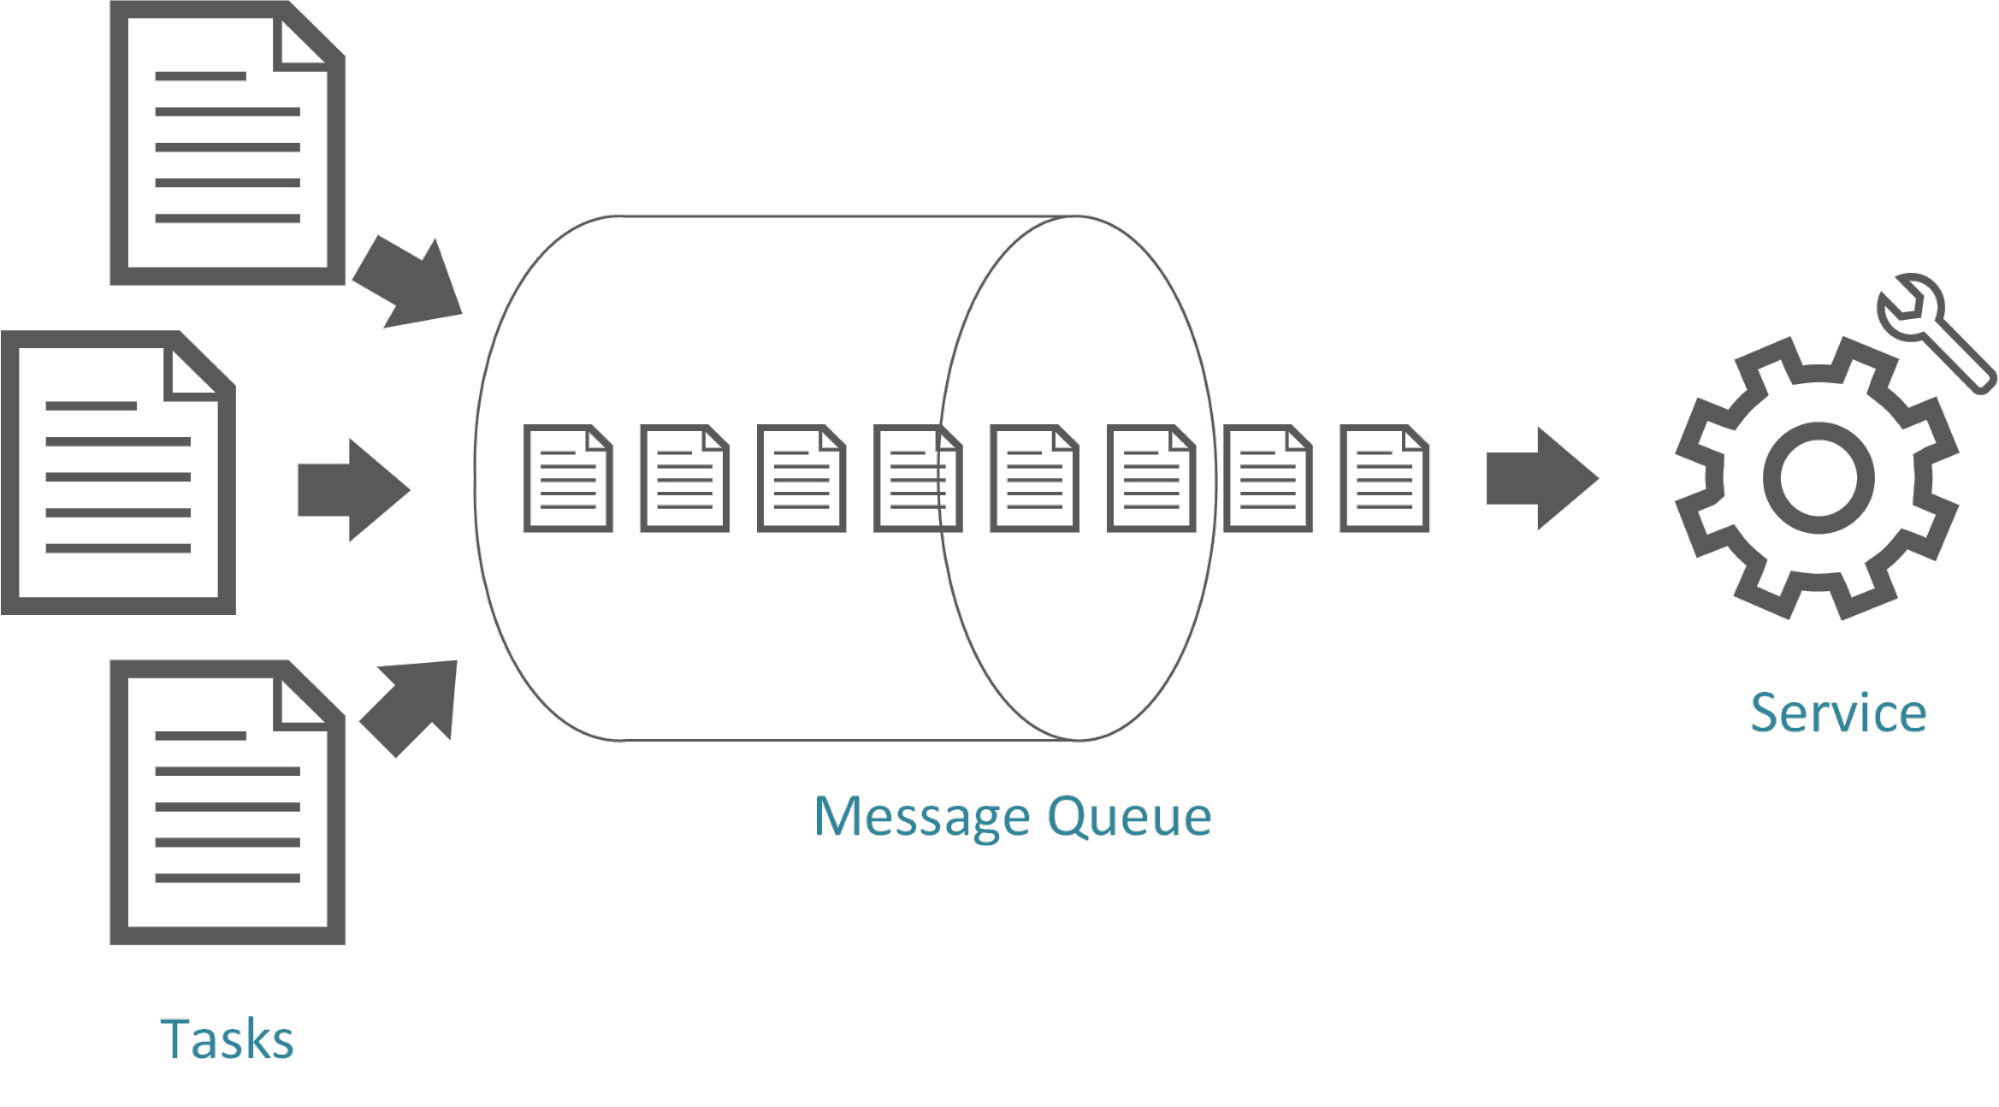
\includegraphics[width=\linewidth]{task_worker}
    \centering
    \caption{Tasks Worker}
    \label{fig:task_worker}
\end{figure}

\end{itemize}

\section{Variables}

Variables are the way to store data in The BPM and are used to exchange data between different tasks
and nodes.\\\\
Variables can be one of these data types
\begin{itemize}
    \item Booleans
    \item Strings
    \item Numbers
\end{itemize}
Many nodes have input and output fields that can be assigned to a variable that can change how this
node will behave.

\section{The BPM Cycle}

As stated before BPM works in a cycle and we will see how this cycle is executed in The BPM to execute business processes.
\\\\
The first thing the business will need to decide the business rules after deciding on the business rules the business will use our suit of applications.\\\\
Each Application works as stand alone application to execute part of the BPM cycle

\subsection{Designer}
\begin{figure}[h]
    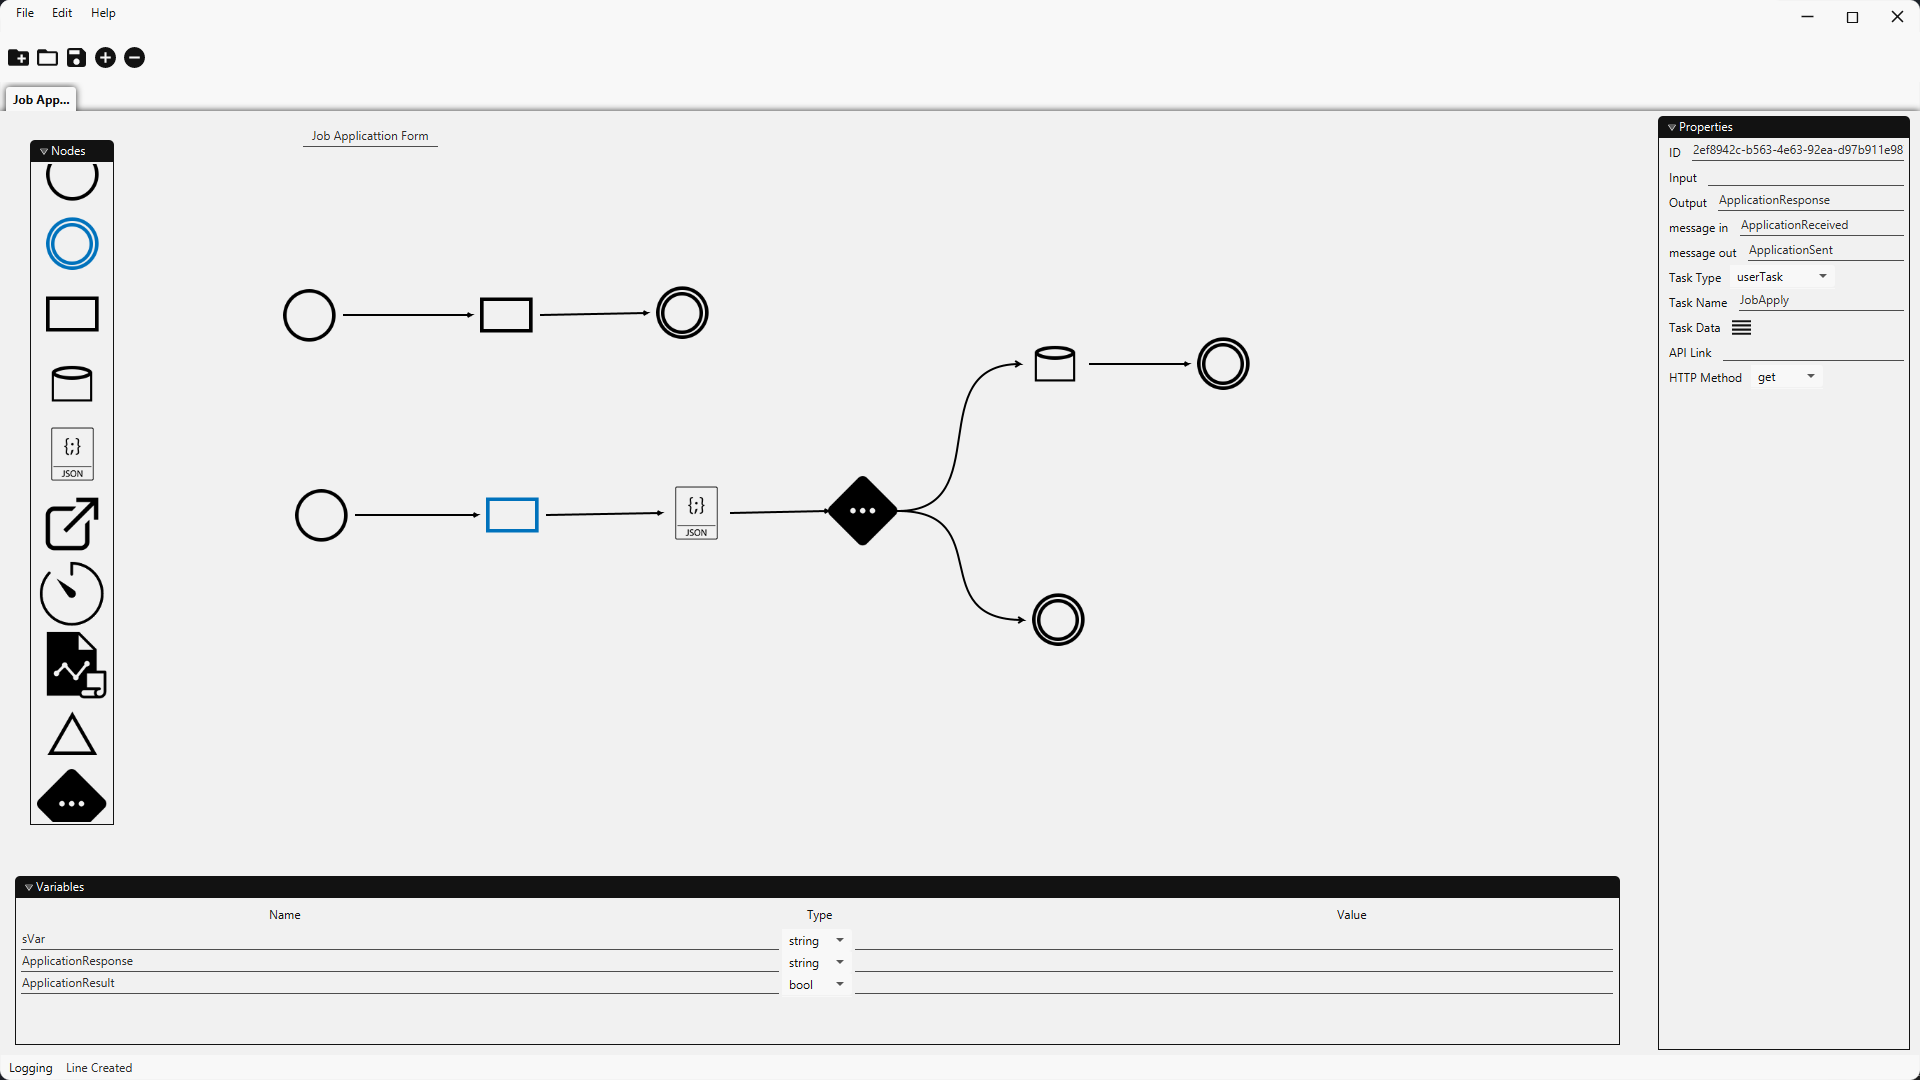
\includegraphics[width=\linewidth]{designer3}
    \centering
    \caption{Designer}
    \label{fig:designer}
\end{figure}

The designer is used to design the business process and adding variables to be initialized at run time
and modify how each node will behave.
It includes

\begin{itemize}
    \item A SQL editor to format SQL query for Database node, request editor for service task node
    \item A JSON Editor to define request or objects in JSON format and can also be used to read
    \item A User task editor to define tasks that need to be done by human actors
\end{itemize}

The designer enables the user to design the workflow, add variables to be added to run time and
properties window to change the nodes setting.\\\\
The process is then generated in an XML file format and the file is now ready for the engine to load
and execute.\\\\
Tools used to build designer
\begin{itemize}
    \item Java
    \item JavaFX 11 used to build the GUI as it allows you to create Java applications with a
    modern, hardware-accelerated user interface that is highly portable
    \item Gradle as a build system
\end{itemize}

\subsection{Engine}

The main system in the engine is the workflow engine which is used to execute the process by moving
the flow of execution from one node to another.\\\\
A workflow engine manages and monitors the state of activities in a workflow, such as the processing
and approval of a loan application form, and determines which new activity to transition to according
to defined processes (workflows). The actions may be anything from saving an application form in a
document management system to send a reminder email to users or escalating overdue items to
management. A workflow engine facilitates the flow of information, tasks, and events. Workflow
engines may also be referred to as Workflow Orchestration Engines.\\\\
Workflow engines mainly have these functions

\begin{itemize}
    \item Verification of the current process status: Check whether it is valid to execute a task, given
    current status
    \item Determine the authority of users - Check if the current user is permitted to execute the task
    \item Executing condition script: After passing the previous two steps, the workflow engine
    executes the task, and if the execution is completed successfully, it returns the success, if not,
    it reports the error to trigger and roll back the change
    \item A workflow engine is a core technique for task allocation software, such as business process
    management, in which the workflow engine allocates tasks to different executors while
    communicating data among participants. A workflow engine can execute any arbitrary
    sequence of steps, for example, a healthcare data analysis
\end{itemize}

The Engine has an API that enables other applications to use its functions and integrate them into their
systems and it is what the ERP uses to integrate The BPM inside it.\\\\

The API gives other applications the ability to manipulate workflow
\begin{itemize}
    \item Load, Start, alter and stop execution
    \item Get the tasks
\end{itemize}

Tools used to build engine
\begin{itemize}
    \item Java
    \item Gradle as a build system
\end{itemize}


\subsection{Monitor}

The Monitor is used to follow the execution of a process and can modify its execution, it helps give
users the ability to view the process and monitor it if anything went wrong or if there is a
bottlenecking anywhere in the process that needs to be modified and get an idea of how the process is
going\\\\
Tools used to build monitor
\begin{adjustwidth}{2cm}{}
    .Net core to be integrated easily with The ERP application\\
\end{adjustwidth}

\chapter{BPM Examples}

\section{Examples of Process-Based Applications}
The following examples are familiar to many organizations.\\\\
We will start with a simple example that shows how to model a simple business process.

\subsection{Bakery}
We want to model the following situation using BPMN 2.0. For a bakery which will start at the
beginning of each day. They will start by baking the bread then selling it and at the end of the day, all
the workers will receive their payments.

\begin{figure}[h]
    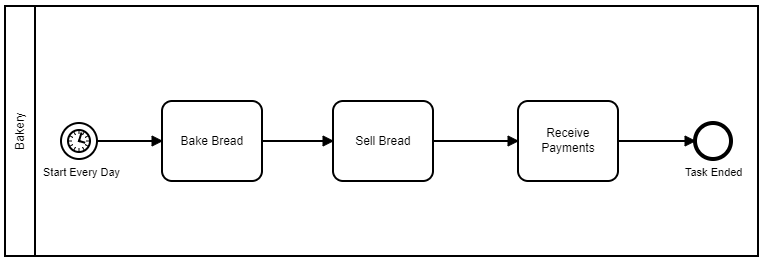
\includegraphics[width=100mm]{bakery}
    \centering
    \caption{Bakery Worflow}
    \label{fig:bakery}
\end{figure}

For our Implementation 
\begin{figure}[h]
    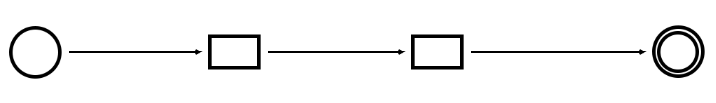
\includegraphics[width=100mm]{bpm_bakery}
    \centering
    \caption{Bakery Worflow}
    \label{fig:bpm_bakery}
\end{figure}

It will be the same as the BPMN 2.0 design for the notations but the difference of how to achieve tasks.\\
For our implementation the tasks needs to be defined somewhere like in the business system or to exist through an API or external tasks in the system.


\subsection{Payment Request}
We will use the following example to illustrate how to model a two-step escalation using BPMN 2.0.
When we want a pizza, we order one. Sometimes the pizza delivery screws up and the delivery takes
longer than 20 minutes. Then we complain to the delivery service. After that, we give them another 30
minutes to deliver the pizza. If they do not make it in time, we give up and cancel our order.

\begin{figure}[h]
    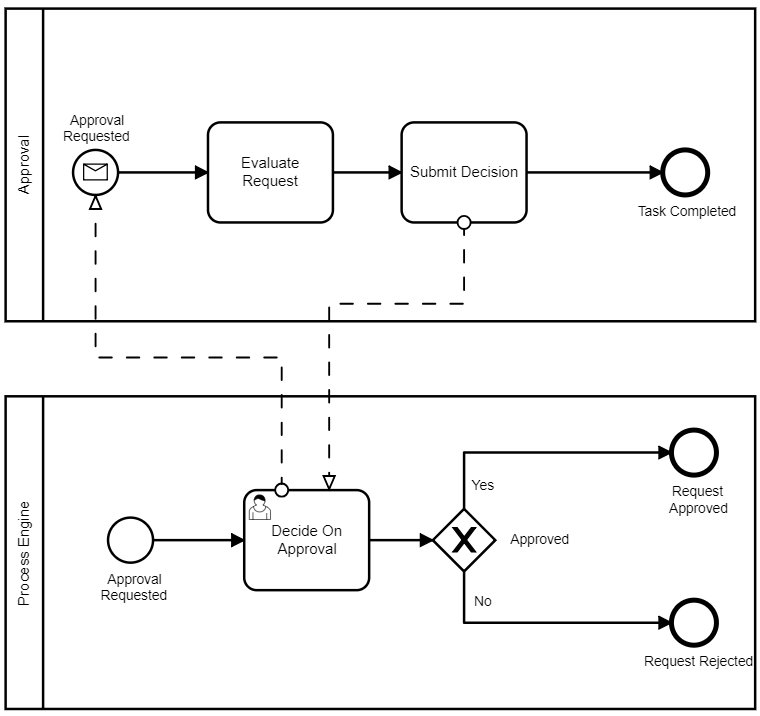
\includegraphics[width=80mm]{payment}
    \centering
    \caption{Payment Request Worflow}
    \label{fig:payment}
\end{figure}

For our Implementation
\begin{figure}[h]
    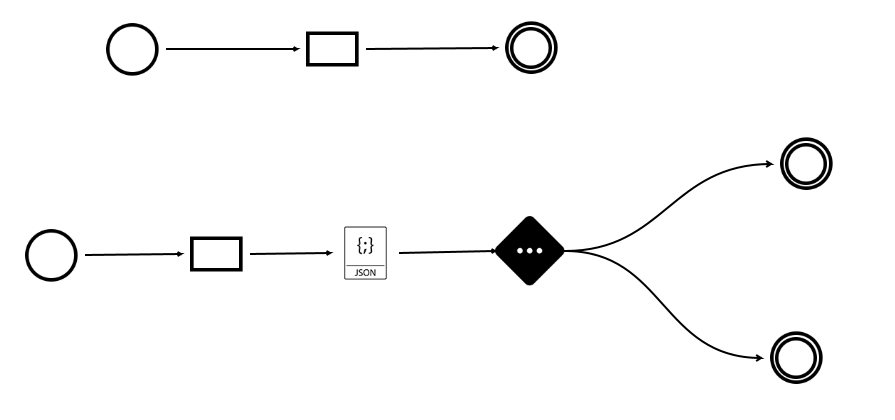
\includegraphics[width=120mm]{bpm_payment}
    \centering
    \caption{Bakery Worflow}
    \label{fig:bpm_payment}
\end{figure}

The messages will be defined in the properties and each task task that wants to send message will add it  in the properties and the nodes listening to this message 
will start to work. In our example this will be the start node at the top will be waiting for a message from a task to start\\\\
Our Workflow still works in the same matter as BPMN 2.0 the difference will be the addon of json node which we need to deal with different requests 
as the user task will have the respond from the person who will evaluate the request.\\\\
As for the BPMN 2.0 handling the request will be through code and they will upload the handling to the engine. But for us to make it easy to use we wanted to handle requests 
through the designer which is used here to check what the payment evaluation will be which will the condition node use to decide which way to go.

    \part{Hardware}
    \chapter{The Factory}
The Factory is a separate project that represents a business model with certain needs for the business
to succeed and make profits.\\\\
The business model involves business processes that are the core of this business. These processes
include
\begin{itemize}
    \item Manufacturing the products
    \item Warehousing
    \item Provide an online market to show the products and sell them
    \item Delivering the products to the customers
\end{itemize}

The Factory is made as a prototype of a business that wants to include technologies in their business
like
\begin{itemize}
    \item IOT
    \item Factory 4.0
    \item Provide an online market to show the products and sell them
    \item Delivering the products to the customers
\end{itemize}

The main purpose of The Factory project is to show a migration of an existing business with an
already working business model with The ERP and The BPM and how the business benefits by
migrating the business with our solutions.\\\\
We will first discuss The Factory as a separate project, its components, and how it works. Then we
will have a look at how migration can be done.\\\\
A flow diagram that shows how The Factory works in a separate matter Fig \ref{fig:factory_flow}\\\\

The factory flow will work when a user make an order which will be uploaded to the cloud which will notify the system and then a user will evaluate if agreed it will send it to the 
Hardware to start make the order.

\begin{figure}[h]
    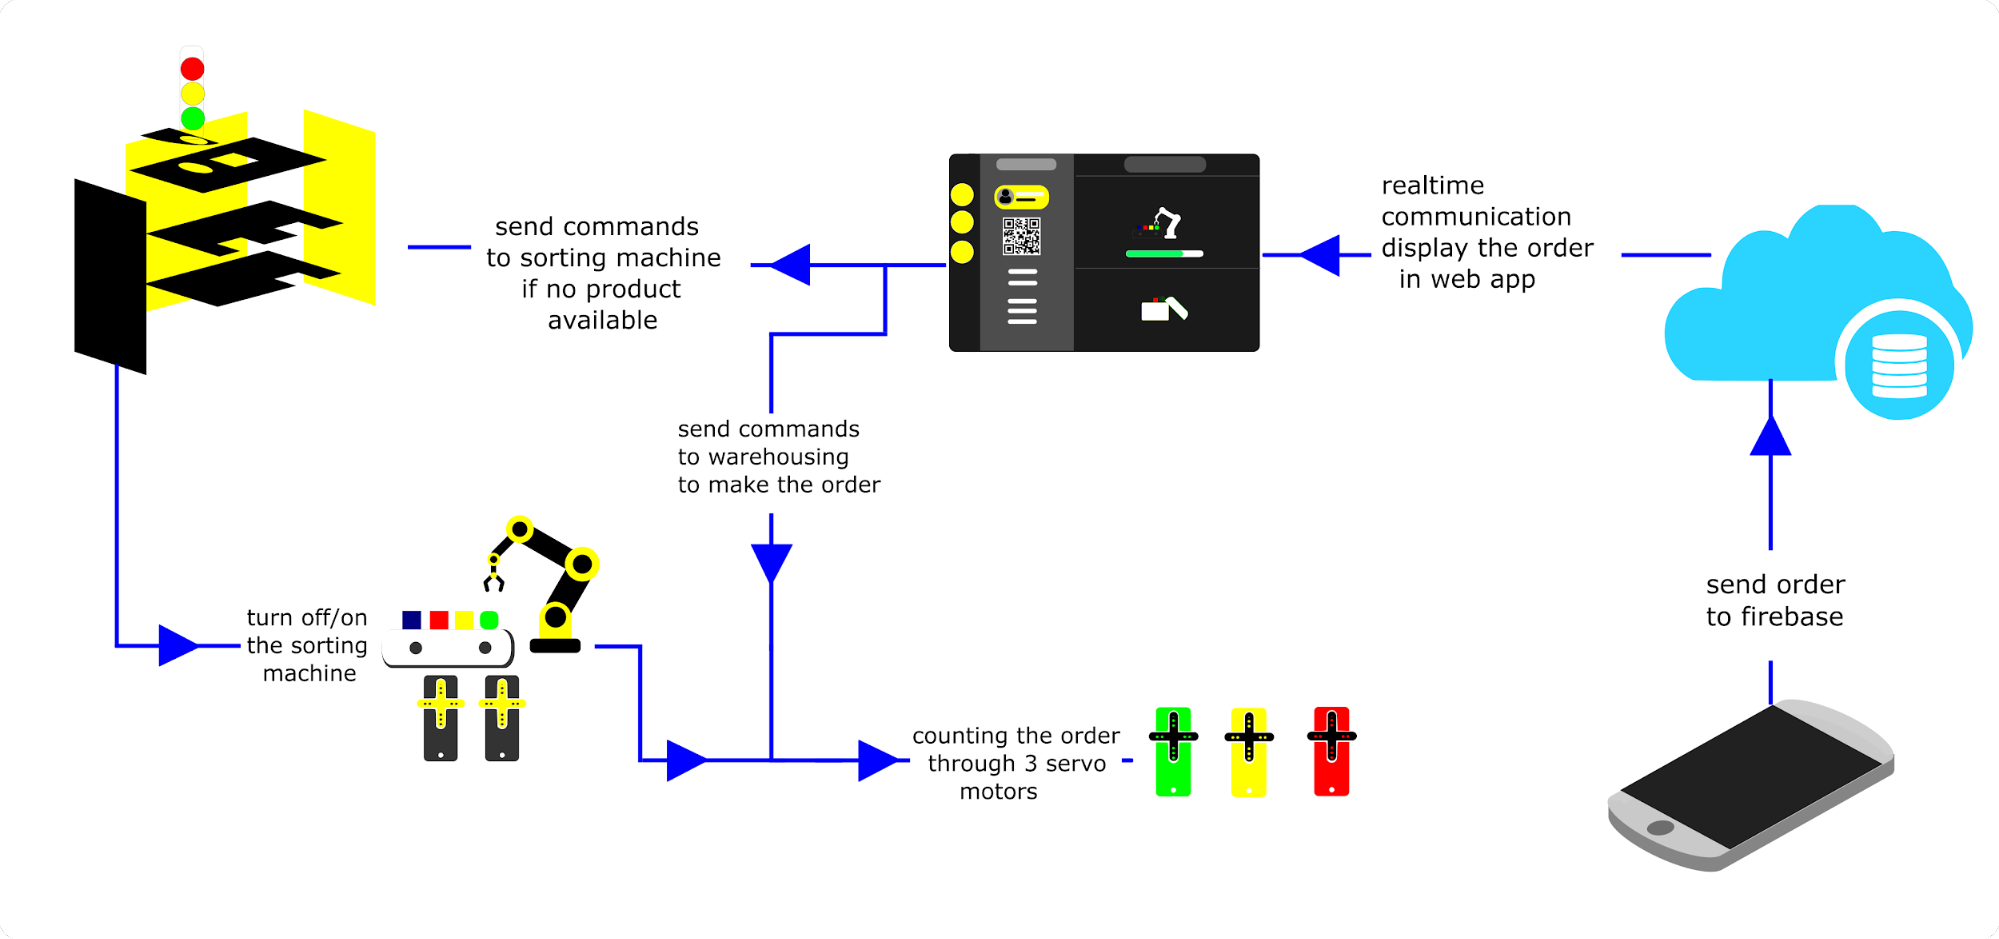
\includegraphics[width=\linewidth]{factory_flow}
    \centering
    \caption{The Factory Flow}
    \label{fig:factory_flow}
\end{figure}


\chapter{Hardware}

\section{Factory box Design}
We made all the factory box from black and yellow acrylic sheet with thickness 3 mm with a press fit
design to make assembling easier.\\
First, there are many programs used to make 3d designs like SolidWorks or Inventor but we used
CorelDRAW 2d program. It is a vector graphics editor that exports DXF files that the CNC machine
uses to execute the design.\\
It consists of three main parts. Fig \ref{fig:hard1}
\begin{itemize}
    \item Sorting part
    \item Warehousing part
    \item Collecting part
\end{itemize}

\begin{figure}[h]
    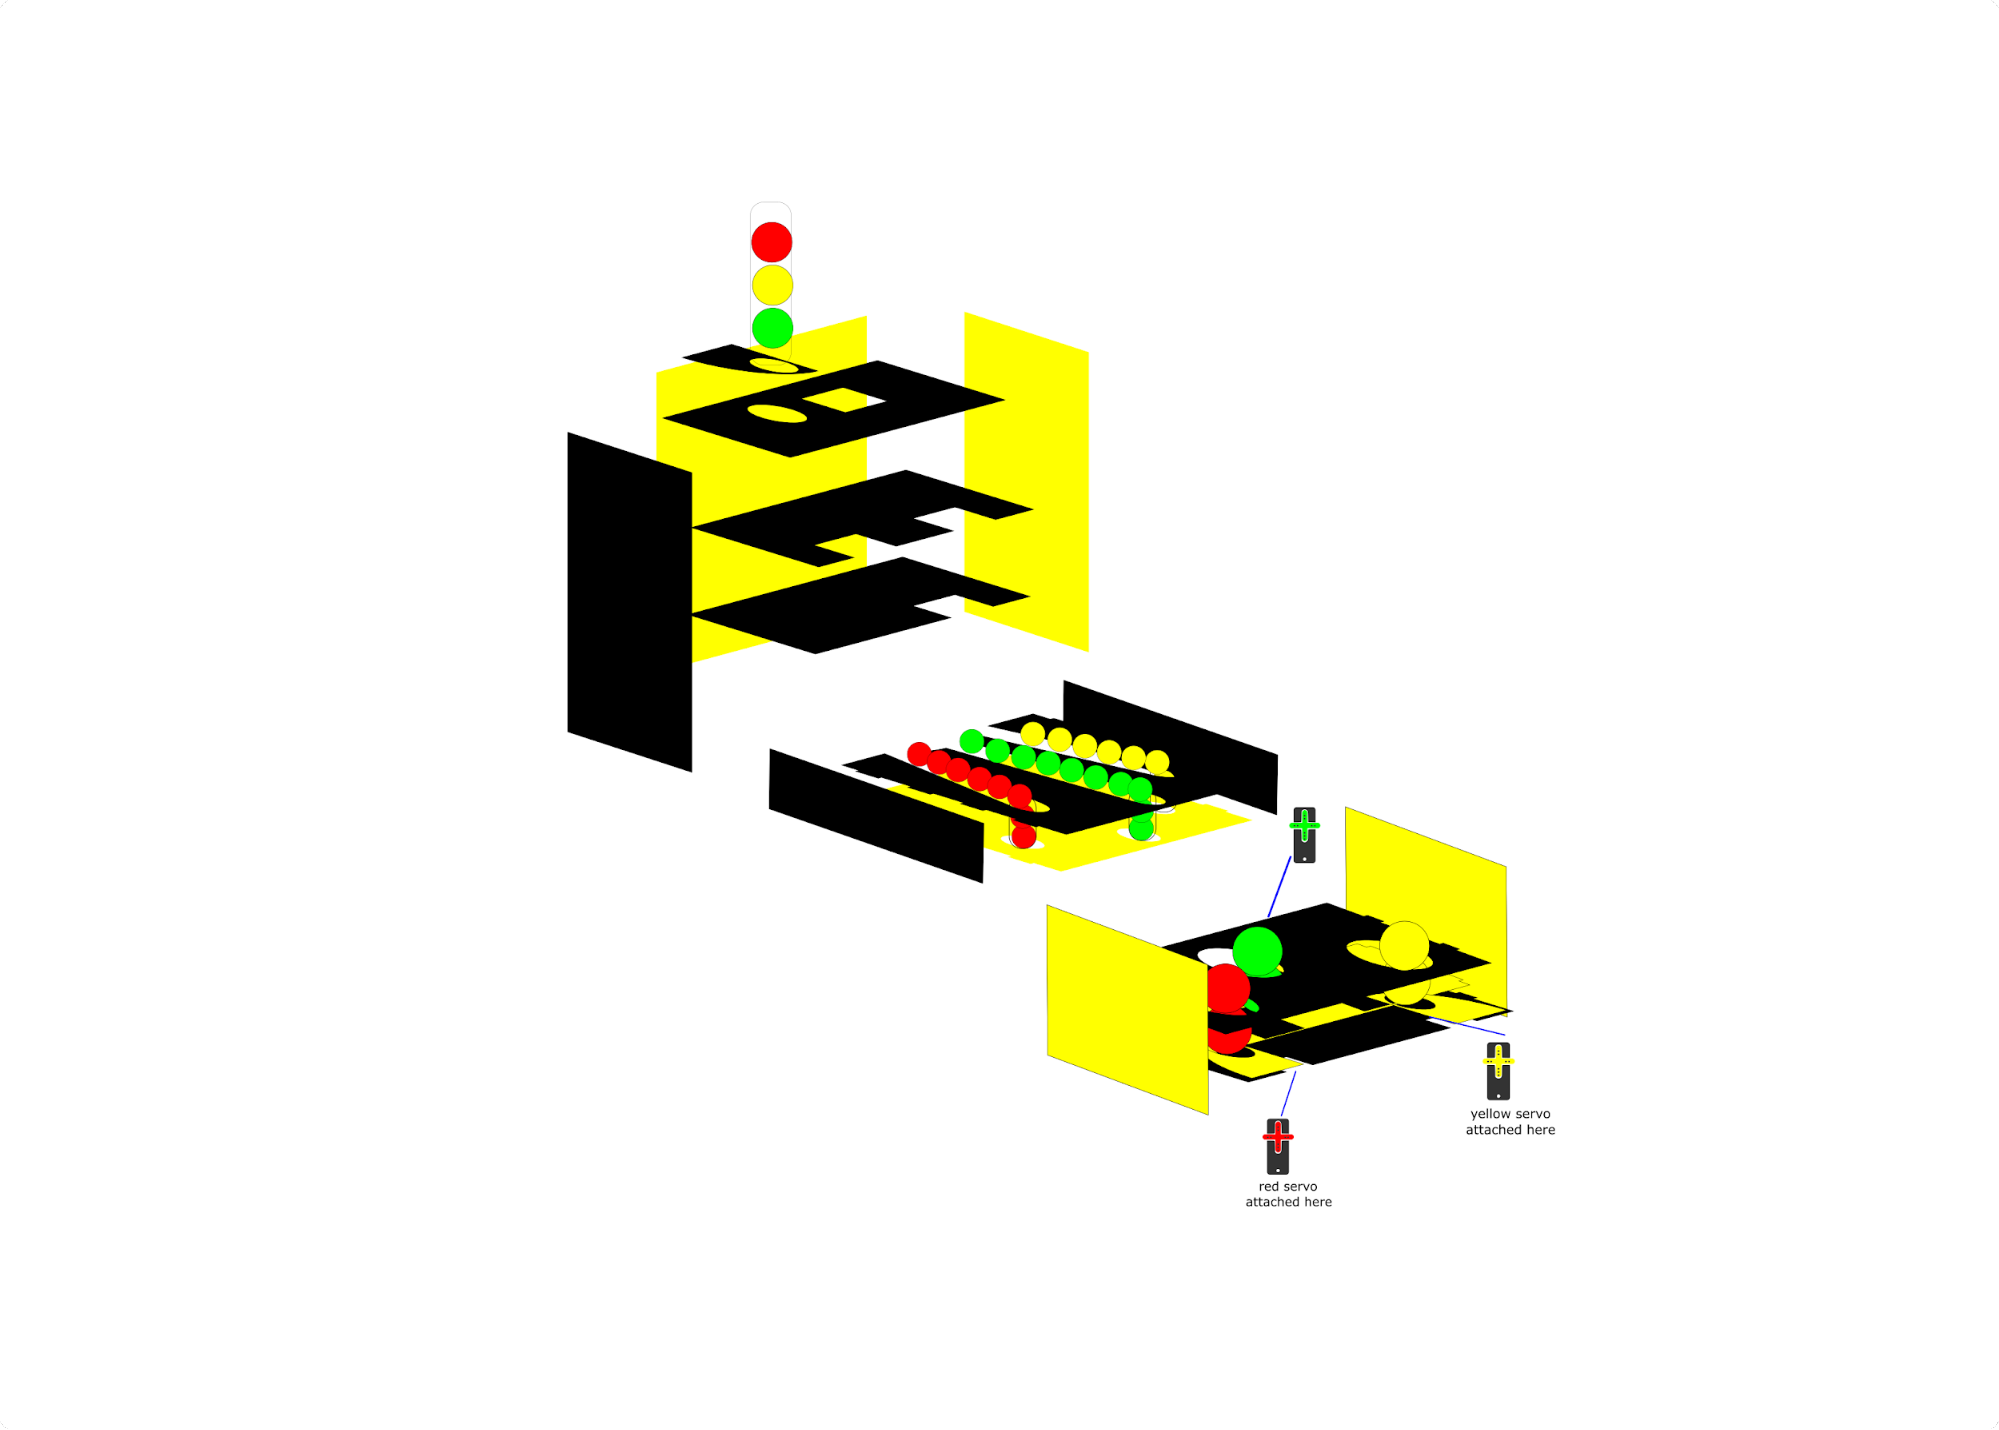
\includegraphics[width=105mm]{hard1}
    \centering
    \caption{Factory Box}
    \label{fig:hard1}
\end{figure}

\subsection{The sorting part}
This part is considered the first stage of our factory. The aim of this part is to make sorting to our
spherical products (colored ball) based on their colors then put them in a fixed place to bring them
quickly.\\
The base of this frame is a (10 cm * 15 cm) and the height is 30 cm.\\
It has 2 servo motors (upper and lower) and one color sensor. The upper servo takes the ball from the
cylindrical tube to put it below the sensor, so the sensor detects its color and the lower servo moves
the ball to the second stage in a specific route. Fig \ref{fig:hard2}

\begin{figure}[h]
    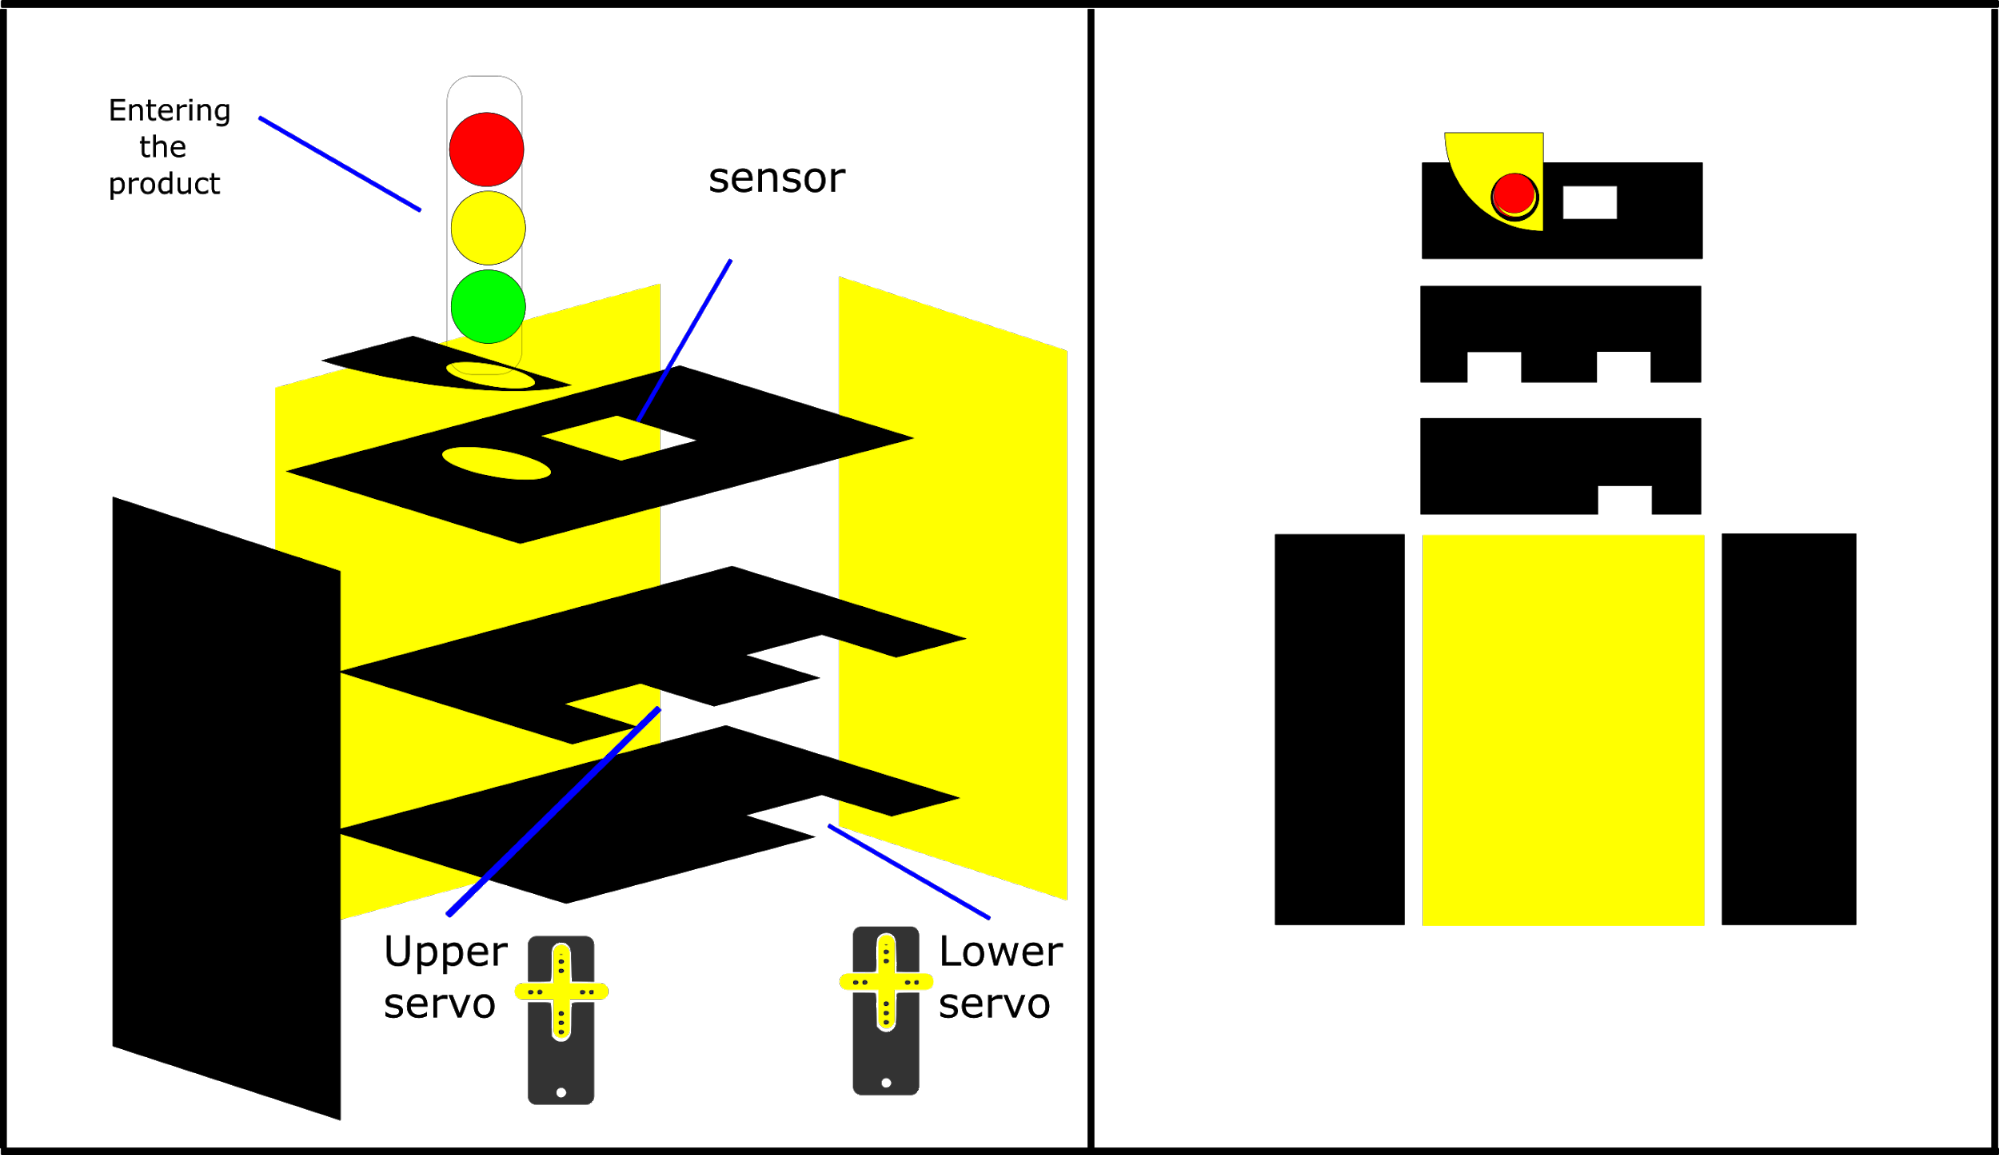
\includegraphics[width=100mm, height= 50mm]{hard2}
    \centering
    \caption{Sorting Part}
    \label{fig:hard2}
\end{figure}


\subsection{Warehousing part}
This part is considered the second stage. The aim of this part is to store the balls in a specific route
based on their colors.\\
We made the route slightly leaning forward to make the motion of the ball smooth.
There is a hole at the end of the route to drop it to the third stage.\\
The base of this part is a (20 cm * 15 cm) and the height is 5 cm. Fig \ref{fig:hard3}

\begin{figure}[h]
    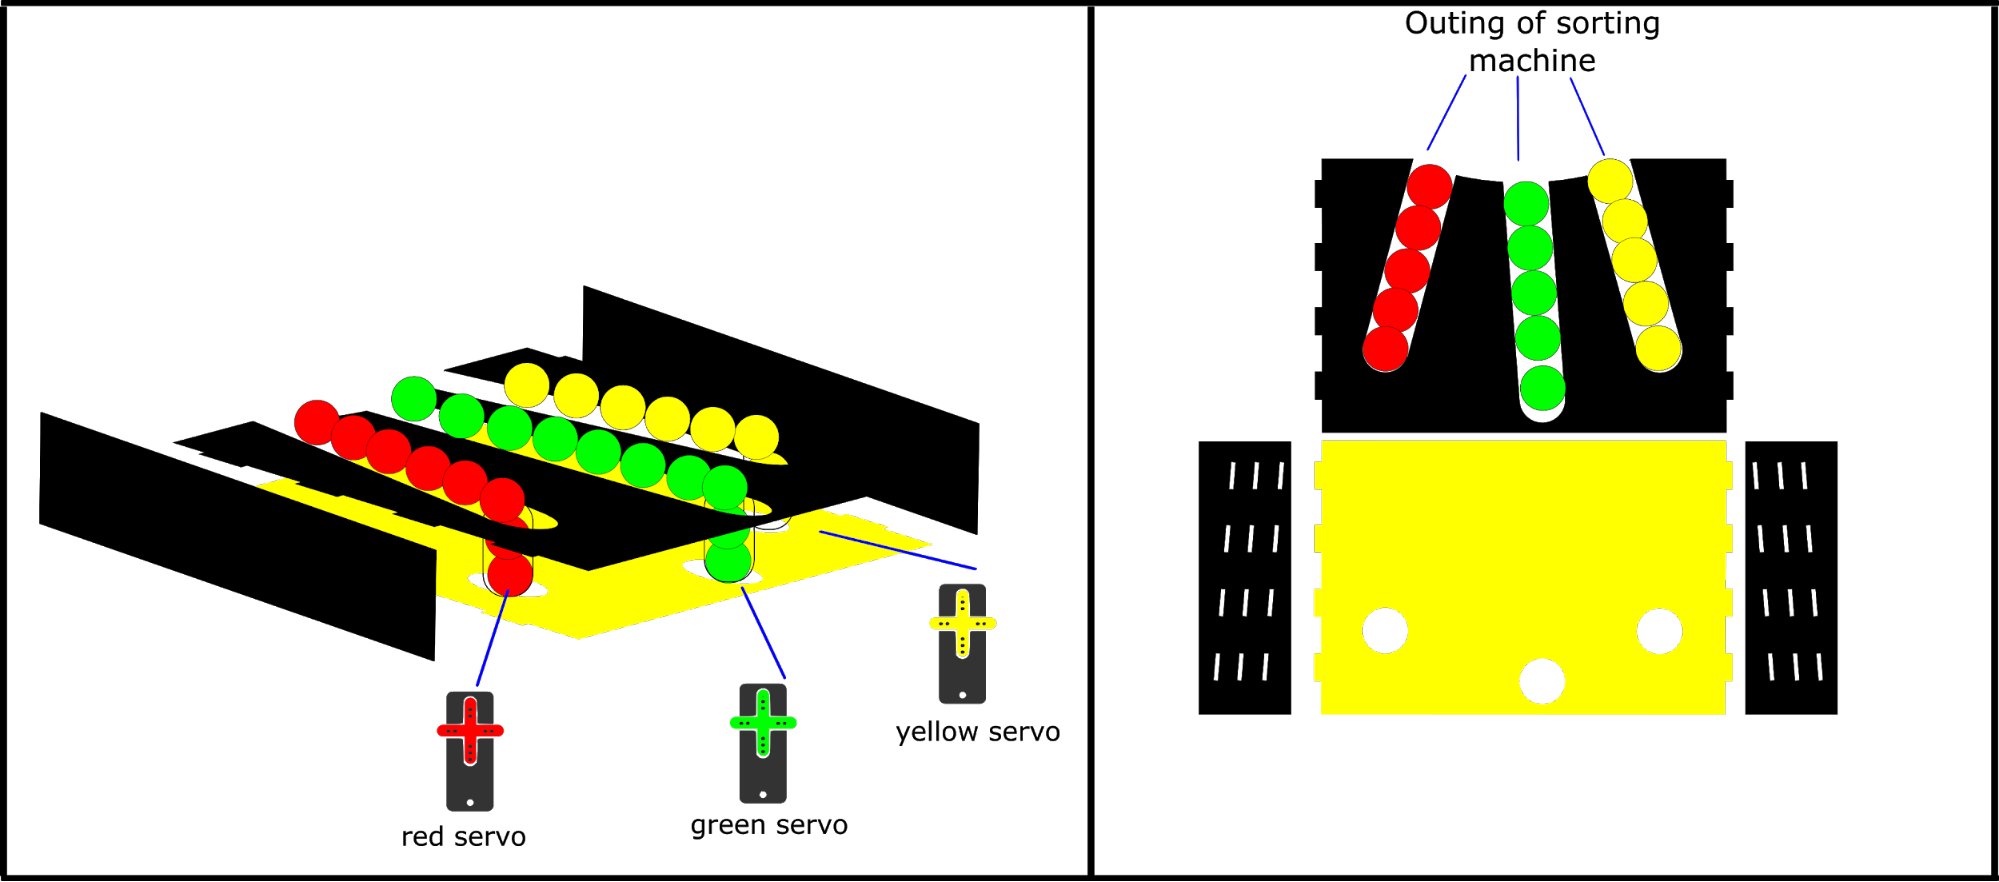
\includegraphics[width=100mm, height=35mm]{hard3}
    \centering
    \caption{Warehousing Part}
    \label{fig:hard3}
\end{figure}

\subsection{Collecting part}
This part is considered the third stage. The aim of this part is to take the product from the warehousing
stage and drop it down to the delivery box.\\
It has 3 servo motor as we have 3 colors in the warehousing, each servo motor moves with a specific
angle to drop down the ball into the box and return to the first angle to take the second ball ..etc\\
The base of this part is a (20 cm * 10 cm) and the height is 10 cm. Fig \ref{fig:hard4}

\begin{figure}[h]
    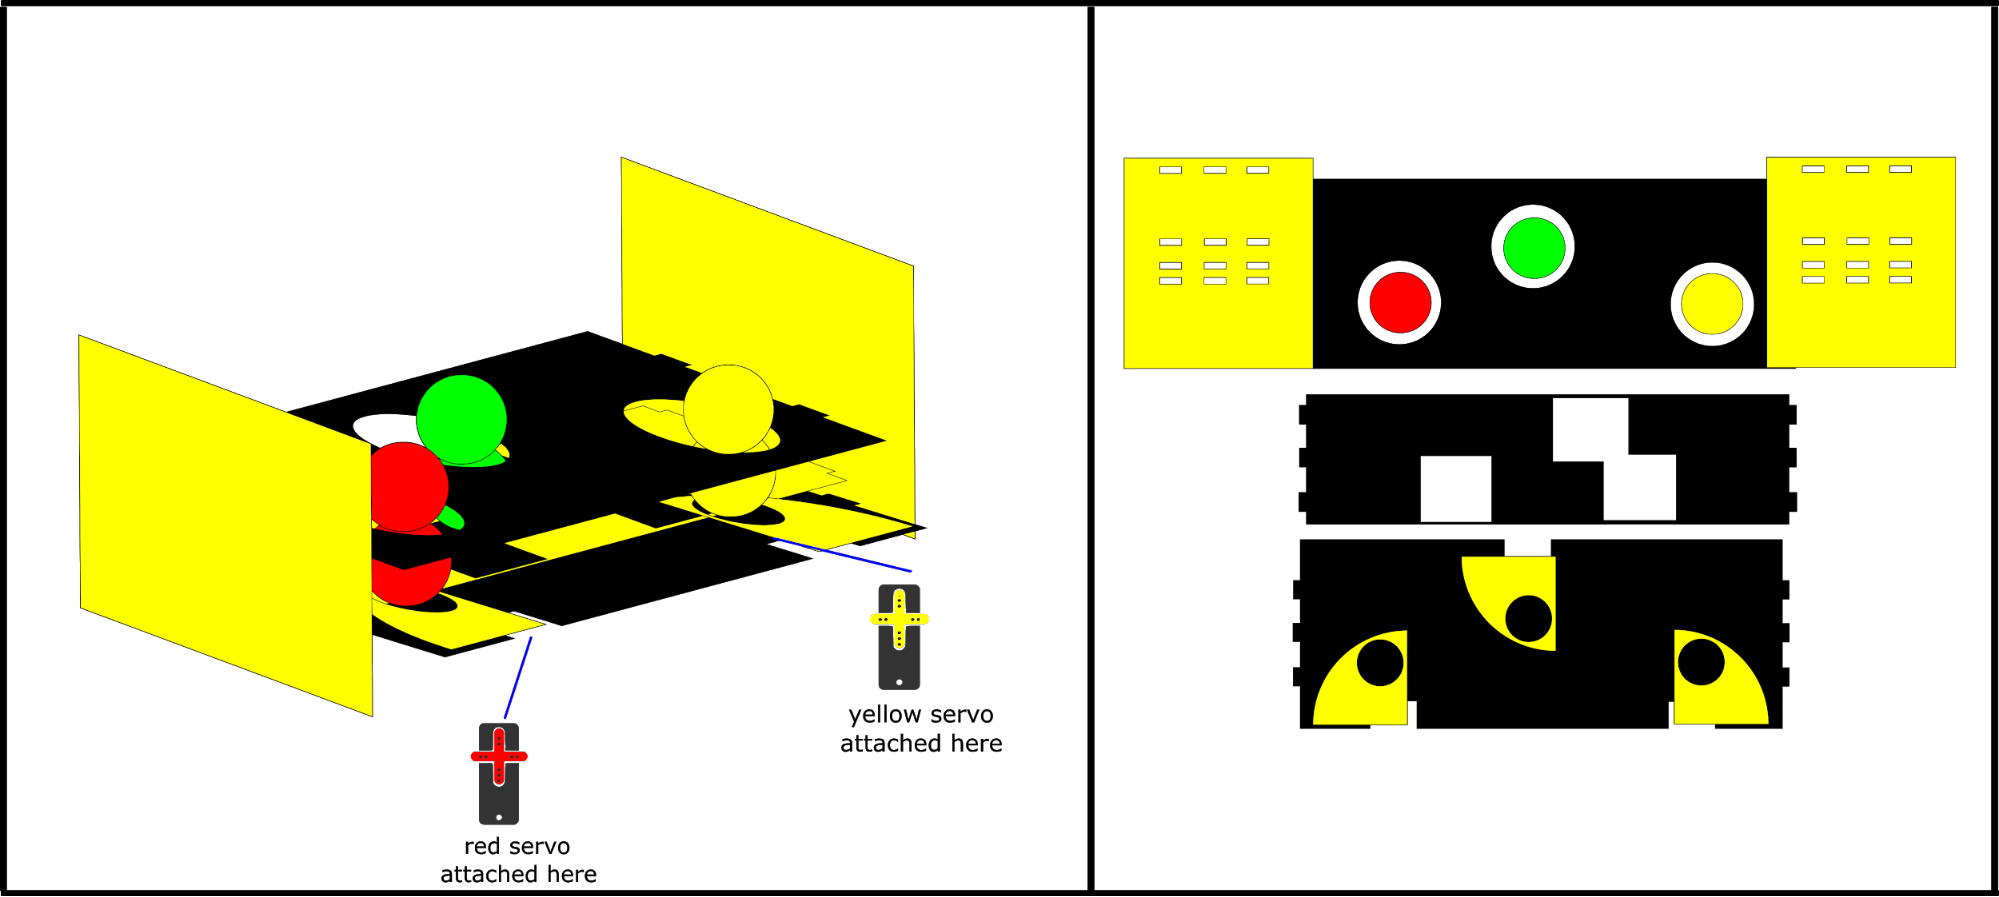
\includegraphics[width=100mm, height=35mm]{hard4}
    \centering
    \caption{Collecting Part}
    \label{fig:hard4}
\end{figure}

\subsection{The Base}
Finally, This part is made to collect the other parts on it.\\
The base of this part is a (40 cm * 35 cm) and the height is 10 cm. Fig \ref{fig:hard5}

\begin{figure}[h]
    
\includegraphics[width=100mm, height=35mm]{hard5}
    \centering
    \caption{The Base}
    \label{fig:hard5}
\end{figure}

\section{components used}

\begin{itemize}
    \item TCS230 RGB Color Sensor
    \item Servo Motor
    \item Arduino Uno
    \item Node MCU
\end{itemize}

\subsection{TCS230 RGB Color Sensor}

\begin{wrapfigure}{r}{0.25\textwidth}
    \begin{center}
      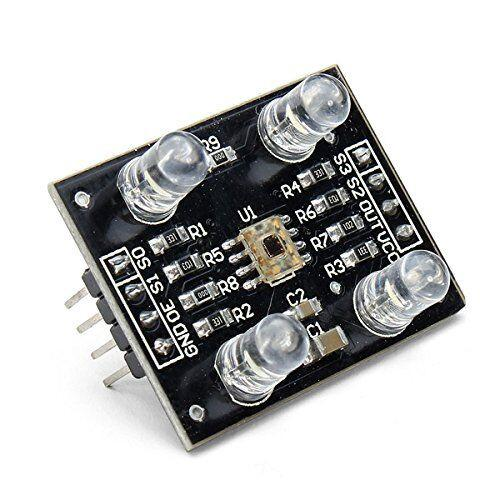
\includegraphics[width=0.25\textwidth]{node}
    \end{center}
  \end{wrapfigure}

The TCS230 senses color light with the help of an 8*8 array of
photodiodes.\\
Then using a Current-to-Frequency Converter the readings from the
photodiodes are converted into a square wave with a frequency directly
proportional to the light intensity.\\
Finally, using the Arduino Board we can read the square wave output and
get the results for the color.\\\\

\begin{center}
    
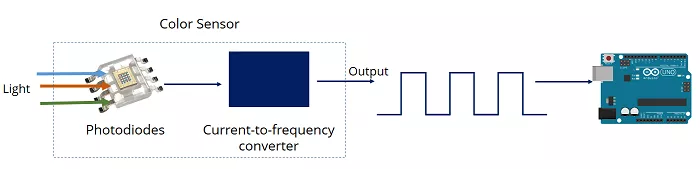
\includegraphics[width=\linewidth]{color_sensor}
\end{center}

\begin{wrapfigure}{r}{0.25\textwidth}
    \begin{center}
      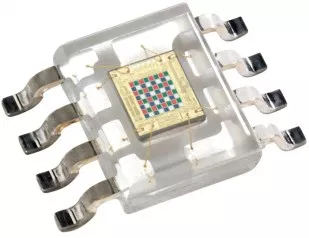
\includegraphics[width=0.25\textwidth]{node2}
    \end{center}
  \end{wrapfigure}

  If we take a closer look at the sensor we can see how it detects various colors.
  The photodiodes have three different color filters.\\
  Sixteen of them have red filters, another 16 have green filters, another 16 have
  blue filters and the other 16 photodiodes are clear with no filters.\\\\\\

  The 16 photodiodes are connected in parallel. Using the two control pins S2 and S3 we can select
which of them will be read. For example, if we want to detect red color, we can just use the 16 red
filtered photodiodes by setting the two pins to LOW logic level according to the table.\\\\
The sensor has two more control pins, S0 and S1, which are used for scaling the output frequency.
The frequency can be scaled to three different preset values of 100\%, 20\%, or 2\%.
This frequency-scaling function allows the output of the sensor to be optimized for various frequency
counters or microcontrollers.

\begin{center}
    
    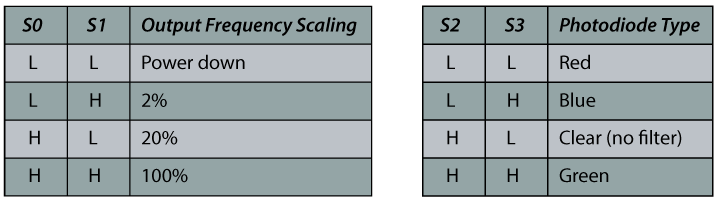
\includegraphics[width=\linewidth]{node_data}
    \end{center}

\subsection{Servo motor}

\begin{wrapfigure}{r}{0.25\textwidth}
    \begin{center}
      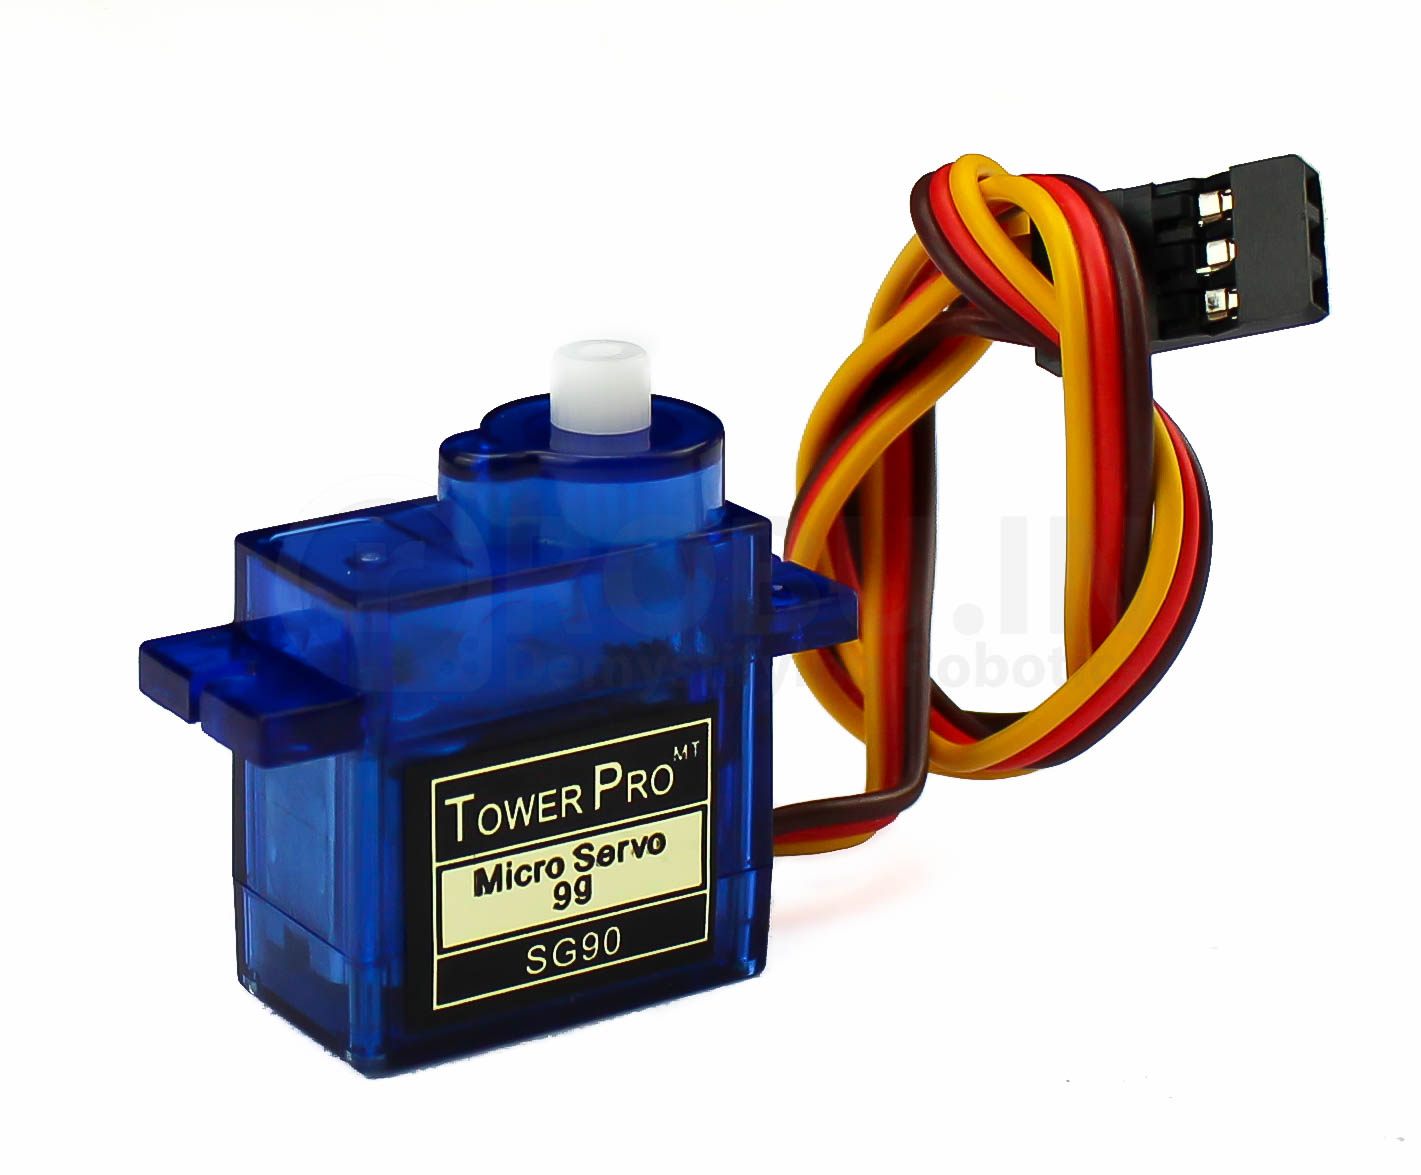
\includegraphics[width=0.25\textwidth]{servo}
    \end{center}
  \end{wrapfigure}

A servo motor is a closed loop servomechanism that uses position feedback to
control its motion and final position. The input to its control is a signal
(analog or digital) representing the position commanded for the output shaft.\\\\
Controlling a servo motor directly from the Arduino is quite easy. However,
a servo motor may require significantly more current than the Arduino can
provide. So we used an external power supply to provide the required current
to the servo motor.\\\\
We used 2 servo motors in the sorting part (upper and lower servo) and 3
servo motors in the collecting part (red, green, and yellow servo).

\subsection{Arduino Uno}

\begin{wrapfigure}{r}{0.25\textwidth}
    \begin{center}
      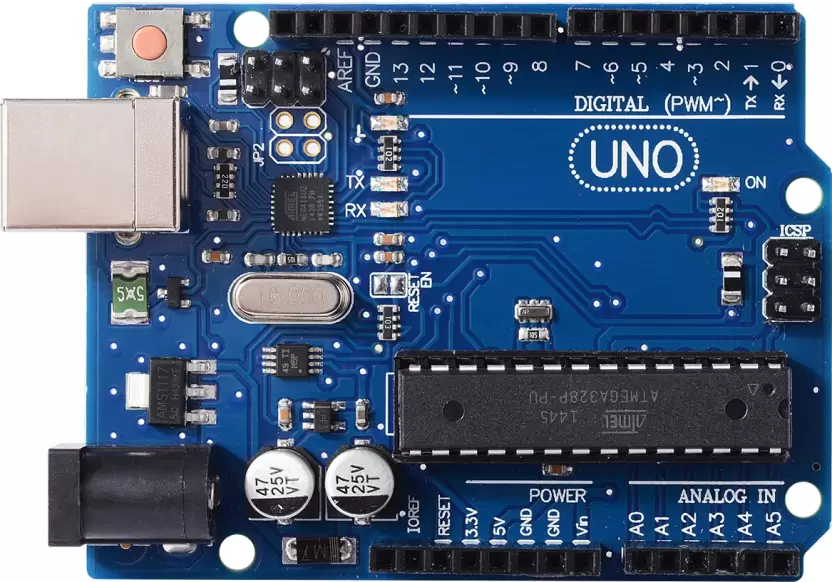
\includegraphics[width=0.25\textwidth]{arduino1}
    \end{center}
  \end{wrapfigure}

  Arduino Uno is a microcontroller board based on the
  ATmega328P. It has 14 digital input/output pins (of which 6
  can be used as PWM outputs), 6 analog inputs, a 16 MHz
  quartz crystal, a USB connection, a power jack, an ICSP
  header, and a reset button.\\\\
  It contains everything needed to support the microcontroller;
  simply connect it to a computer with a USB cable or power it
  with an AC-to-DC adapter or battery to get started.\\\\
  We used Arduino Uno to run the sensor and to control the 2
  servo motors of the sorting part\\


  \begin{figure}[h]
    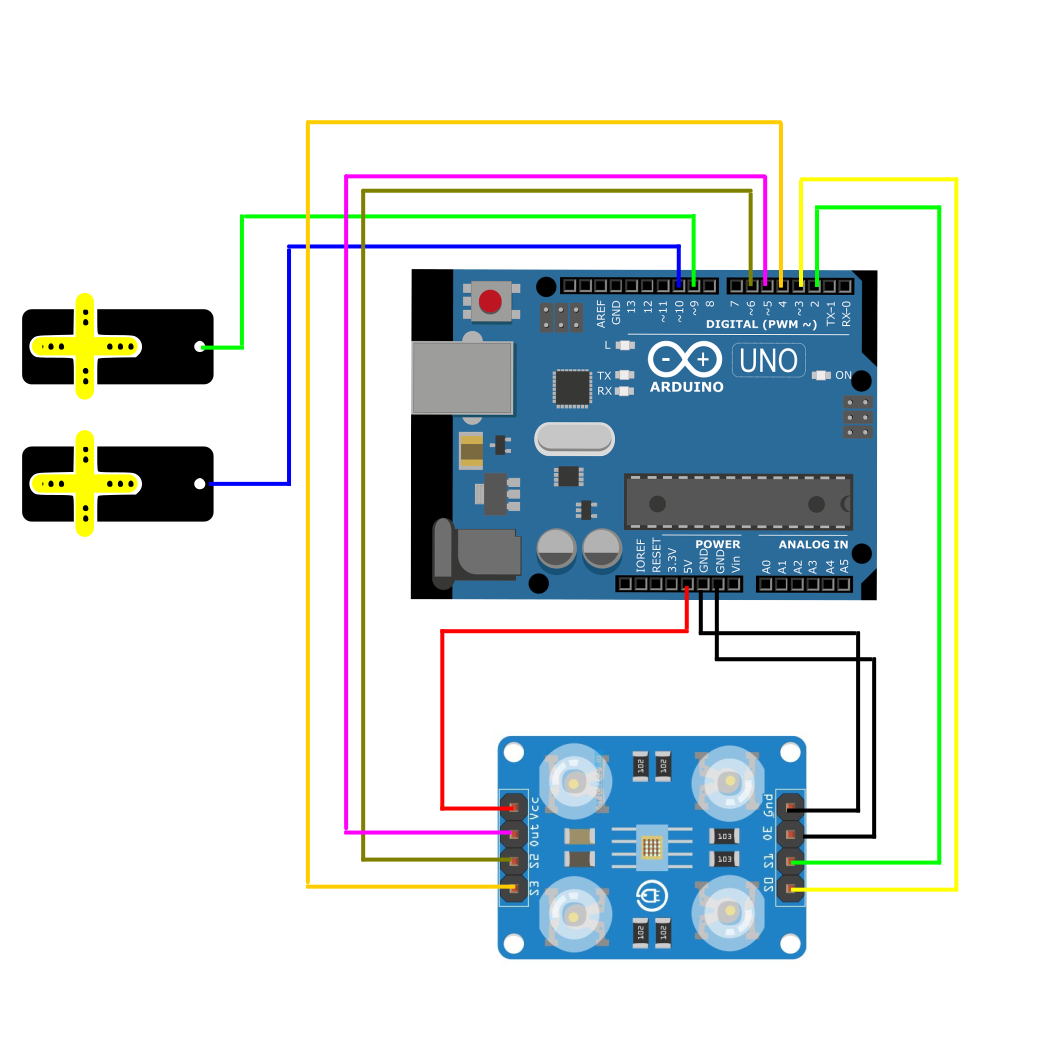
\includegraphics[width=\linewidth]{arduino2}
    \centering
    \caption{Sorting Connection diagram}
    \label{fig:arduino2}
\end{figure}

\subsection{Node MCU}

\begin{wrapfigure}{r}{0.25\textwidth}
    \begin{center}
      \includegraphics[width=0.25\textwidth]{mcu1}
    \end{center}
  \end{wrapfigure}

  In our project, we need wireless communication to connect the Arduino
to the web application, so we used NodeMcu.\\\\
It is an open source IoT platform. It includes firmware which runs on
the ESP 8266 Wi-FI SOC.\\\\
We also used it to control the 3 servo motors of the collecting part as it
has PWM output pins.\\\\
We used serial communication to connect the Arduino to the NodeMcu
to exchange the data between them.\\

\begin{figure}[h]
    \includegraphics[width=\linewidth]{mcu2}
    \centering
    \caption{Collecting Connection diagram}
    \label{fig:arduino2}
\end{figure}


\chapter{Software}

The software will provide a way to have control over the project and visual feedback of the system
overall and offers the products for sale through an online market.\\\\
The software system is divided into three parts
\begin{itemize}
    \item Server Side
    \item Client Side
    \item Mobile Aoolications
\end{itemize}

\section{Server Side}

\begin{center}
    \includegraphics[width=\linewidth]{server}
  \end{center}

  A server is a computer program or a device that provides functionality for other programs or devices,
called "clients". This architecture is called the client-server model. A server should be reachable from
a user's local computer, smartphone, or other devices. Operations may be performed in server-side
because they require access to information or functionality that is not available on the client, or
because performing such operations on the client side would be slow, unreliable, or insecure.\\\\
The Factory software is built upon this architecture, where the server provides an API to be accessed
by the clients using it.\\\\
The server also talks to the hardware using Socket for real-time, bi-directional communication
between clients (Node MCU in our case) and the server.\\\\
The server API provides
\begin{itemize}
    \item User Authentication, it will validate the user signing in the system
    \item User Data, it will get the data related to the user
    \item Getting the orders
    \item Sending the order to the hardware
\end{itemize}

All connections to the database are done using the server. The database used is firebase, which is a
cloud database solution that helps to quickly develop high-quality apps and grow the business. Data is
stored as JSON and synchronized in real-time to every connected client.\\\\
The server uses the database to store data about
\begin{itemize}
    \item Users of the system
    \item Clients
    \item Orders
    \item Drivers (Which we will discuss their purpose later in the book)
\end{itemize}

\section{Client Side}

\begin{center}
    \includegraphics[width=\linewidth]{client}
\end{center}
The client-side refers to a computer application, such as a web browser, that runs on a user's local
computer, smartphone, or other devices, and connects to a server as necessary.\\\\
Client side will provide a way for users of the business to log into the system, control the hardware
and have an overview of the overall business, like the orders made by customers and the state of the
orders.\\\\
The client app will offer these operations
\begin{itemize}
    \item Display the orders in details
    \item Talk to the server API
    \item Sending orders to the hardware via server API. Sending order to hardware to start the
    manufacturing and prepare process, as orders aren’t permitted to start without a user manually
    evaluating the order and then send the order to the hardware
    \item Monitor the order process. Monitor the order allows the process to have feedback on how the
    process is doing or if there is any problem with the system
\end{itemize}

The client app is built using Vue.js which is a progressive framework for building user interfaces and
single web applications.\\\\
Vue.js has these features that will make the developing simpler
\begin{itemize}
    \item Utilizes a virtual DOM
    \item Provides reactive and composable view components
    \item Maintains focus in the core library, with concerns such as routing and global state
    management handled by companion libraries
\end{itemize}


\section{Client App}

Smartphones are no longer just devices for calls, they are also used to send multimedia messages such
as pictures, videos, and emails. Due to the enormous potential of smartphones, these capabilities can
be exploited by multiple applications that benefit the user, so we tried to make simple and useful
applications to our hardware project.\\\\
The aim of this client android application is providing an easy way to make an order from the factory
and track the order until it reaches the customer's location. It also displays all the orders from the
client.\\\\

\textbf{Tools used}
\begin{itemize}
    \item Software Requirements: Android studio, Java
    \item Database: Firebase
\end{itemize}
\textbf{Features}
\begin{itemize}
    \item Provides users authentication
    \item Makes orders
    \item Tracks order location by using google map
    \item Receives notifications about the order
    \item Checks the Qr code of the order
    \item Displays all orders
    \item Provides statistics profile
\end{itemize}

\begin{figure}[h]
    \includegraphics[width=\linewidth]{blue1}
    \centering
    \caption{Process Flow of the Client Application}
    \label{fig:blue1}
\end{figure}

\subsection{QR Code}
A QR code (quick response code) is a type of 2D barcode that is used to provide easy access to
information through smartphones.\\\\
In our android applications, we need to store the order of each customer and the location of the
customer.\\\\
We stored the data we need in a JSON object to extract the data from it in an easy way.\\\\

\par\vspace {4cm}
\begin{wrapfigure}{r}{0.5\textwidth}
    \begin{center}
      \includegraphics[width=0.5\textwidth]{qr}
    \end{center}
  \end{wrapfigure}

\textbf{For example}\\
\small \{
    \begin{adjustwidth}{2cm}{}
    \small Red : 5,\\
    \small Green : 1,\\
    \small Yellow : 1,\\
    \small Latitude : 30.35,\\
    \small Longitude: 30.59\\
    \end{adjustwidth}

    \small \}\\\\\\

    As the order consists of three products (red, green, and
    yellow) and the location of the customer (latitude and
    longitude) that our application uses to get the location on
    google maps.

\subsection{Process Flow}

The process flow of the client application during making the order Fig \ref{fig:blue2}
\begin{itemize}
    \item The client makes an order
    \item The firebase sends the notification order to the web app to collect it
    \item The web app collects the order and puts it in a box with a printed QR code
    \item The delivery service takes the order and delivers it to the client
    \item The client scans the QR code of the order
    \item The client app displays the contents of the box
\end{itemize}

\begin{figure}[h]
    \includegraphics[width=\linewidth]{blue2}
    \centering
    \caption{Making Order Flow}
    \label{fig:blue2}
\end{figure}



\section{Application screens}
\begin{itemize}
    \item Getting the location of the client by using google maps
    In the registration form, when the client presses on the icon of google maps, the app will open
    google maps screen and store the location of the client
    \item Scanning the Qr code of the order when receiving it, then the application will display the
    status of the order if it is the right or wrong order
\end{itemize}

\section{Driver App}

The aim of this driver android application is providing an easy way to get to the final destination of
the order on google maps then deliver it to the client\\
\newpage

\textbf{Tools used}
\begin{itemize}
    \item Software Requirements: Android studio, Java
    \item Database: Firebase
\end{itemize}

\textbf{Features}
\begin{itemize}
    \item Real-time communication
    \item Users authentication
    \item Checks the QR code of the order
    \item Displays the location of the customer
    \item Displays all targeted locations
\end{itemize}


\begin{figure}[h]
    \includegraphics[width=\linewidth]{red1}
    \centering
    \caption{Process Flow of the Driver Application}
    \label{fig:red1}
\end{figure}

\subsection{Process Flow}

The process flow of the driver application during making the order Fig \ref{fig:blue2}
\begin{itemize}
    \item The web app sends a notification to the driver app after finishing the order
    \item The driver scans the QR code of the order
    \item The driver app displays the destination of the order on google maps and draws the shortest
    route between the two locations
\end{itemize}

%\begin{figure}[h]
%    \includegraphics[width=\linewidth]{red2}
%    \centering
%    \caption{Finishing Order Flow}
%    \label{fig:red2}
%\end{figure}

\subsection{Application screens}
\begin{itemize}
    \item Scanning the QR code of the order, then the application will get the latitude and longitude of
    the customer and pass it to google maps activity to display the shortest path between the
    driver and the customer.
\end{itemize}

    \part{Integration}
    \section{High Level Design}
    Project Design

\section{Architecture}
    Architecture
    
    %\part{Appendix}
    %\section{What Is Next}
    What to be made next in the project

\section{Contributing}
    How to contribute

\section{License}
    The License

\section{Credits}
    No One will get Credits because no one helped

\section{Contacts}
    Our Contacts

    \printbibliography[
      heading=bibintoc,
      title={References}
      ]

\end{document}